% FraudShield paper draft (build prompt Part E.13, milestone M11).
% Status: DRAFT. Not reviewed. See README.md in this directory for the rules every number obeys.
\documentclass[11pt]{article}

\usepackage[utf8]{inputenc}
\usepackage[T1]{fontenc}
\usepackage[a4paper,margin=2.5cm]{geometry}
\usepackage{amsmath}
\usepackage{booktabs}
\usepackage{hyperref}
\usepackage{xcolor}

% numbers.tex: every number the paper states, with its provenance.
%
% The claims register gate (docs/research/claims_register.md) applies to every entry: a number
% is MEASURED (commit and run given) or SOURCED (checkable citation given); nothing else may be
% stated. Sections use these macros and never type a result directly; check_numbers.py enforces
% that.
%
%   \meas{x}      MEASURED on main (M2/M3). Printed as is.
%   \prov{x}      MEASURED on a milestone not yet tagged complete. Printed with a dagger. None is
%                 in use: every M4 value was re-verified at m4-complete (72e7790) on 2026-09-22 by
%                 audit_numbers.py and moved to \meas.
%   \srcd{x}      A value fixed by the specification (a threshold or target), not a result.
%   \notyet{Mx}   A result a later milestone produces. Printed in italics as "not yet measured (Mx)".
%
% Data draws (seed 20260917 throughout):
%   6abde44e  1,006,249 rows (claims register header; M3 and the first M4 battery)
%   d8083dbc  1,006,317 rows (dataset/realism_report.md at m4-complete; the PB-61 draw with the
%             pre-registered non-burst variant; the M4 gate and the E1-corrected battery)
% Evidence files are read at the m4-complete tag (72e7790), which is on main; each file begins
% with its own evidence-commit and evidence-tree-state stamp.

\newcommand{\meas}[1]{#1}
% \srcd{x}: SOURCED from the specification (the Part B resolutions of the specification, or the SRS). A
% requirement or threshold, not a result.
\newcommand{\srcd}[1]{#1}
\newcommand{\prov}[1]{#1\textsuperscript{\dag}}
\newcommand{\notyet}[1]{\emph{not yet measured (#1)}}

% ---------------------------------------------------------------------------------------------
% Dataset (M2), main
% ---------------------------------------------------------------------------------------------
% docs/research/claims_register.md (main) header and C-9: draw 6abde44e.
\newcommand{\nRowsDrawA}{\meas{1{,}006{,}249}}
\newcommand{\nSeed}{\meas{20260917}}
% docs/research/sourcing_pass.md "Result": provenance counts after the pass of 2026-09-18.
\newcommand{\nParamsTotal}{\meas{81}}
\newcommand{\nParamsSourced}{\meas{12}}
\newcommand{\nParamsAssumed}{\meas{55}}
\newcommand{\nParamsCalibrated}{\meas{14}}
\newcommand{\nSourceDocs}{\meas{8}}
% docs/research/limitations.md: fraud.yaml parameters.
\newcommand{\nFraudParams}{\meas{25}}
\newcommand{\nFraudParamsChoice}{\meas{21}}
\newcommand{\nFraudParamsCalibrated}{\meas{4}}
% docs/reviews/M2/milestone-review.md "Two minima"; lab_notebook.md 2026-09-18 (M-4).
\newcommand{\nMinRows}{\meas{170{,}000}}
\newcommand{\nDetectorMinRows}{\meas{60{,}000}}
\newcommand{\nMinRowsA}{\meas{169{,}492}}
\newcommand{\nMinRowsB}{\meas{170{,}455}}
\newcommand{\nMinRowsC}{\meas{169{,}972}}
\newcommand{\nMinRowsD}{\meas{170{,}069}}
% claims_register.md C-9 (draw 6abde44e): strongest dataset column and the event-delay channel.
\newcommand{\nColumnMaxAUC}{\meas{0.706}}
\newcommand{\nEventDelayAUC}{\meas{0.730}}
% claims_register.md C-12: account-grouped folds lower merchant_category_code by 0.005.
\newcommand{\nSiblingLeak}{\meas{0.005}}
% claims_register.md C-13: ten seeds at 300,000 rows; residual size dependence.
\newcommand{\nSeedSdSizeSeries}{\meas{0.0055}}
\newcommand{\nSizeSeriesSpan}{\meas{0.065}}
% claims_register.md C-11: event-delay channel before and after PB-56.
\newcommand{\nEventDelayBefore}{\meas{0.758}}
\newcommand{\nEventDelayAfter}{\meas{0.730}}
\newcommand{\nEventDelayShare}{\meas{11\%}}
\newcommand{\nEventDelayBandLow}{\meas{0.68}}
\newcommand{\nEventDelayBandHigh}{\meas{0.74}}

% Draw d8083dbc (dataset/realism_report.md at m4-complete): distribution and split.
\newcommand{\nRowsDrawB}{\meas{1{,}006{,}317}}
\newcommand{\nFraudRateAll}{\meas{0.877\%}}
\newcommand{\nFraudRateTest}{\meas{0.971\%}}
\newcommand{\nLabelNoiseMissed}{\meas{1.55\%}}
\newcommand{\nLabelNoiseFalse}{\meas{1.64\%}}
\newcommand{\nShortcutAUC}{\meas{0.503}}
\newcommand{\nNovelRows}{\meas{73}}
\newcommand{\nTrainRows}{\meas{792{,}162}}
\newcommand{\nValRows}{\meas{101{,}332}}
\newcommand{\nCalRows}{\meas{40{,}700}}
\newcommand{\nEmbargoRows}{\meas{10{,}914}}
\newcommand{\nTestRows}{\meas{101{,}909}}
\newcommand{\nTestSpanDays}{\meas{63.97}}
\newcommand{\nEmbargoDays}{\meas{6.99}}
\newcommand{\nChannelMixDev}{\meas{0.16}}
\newcommand{\nCountryMixDev}{\meas{0.01}}

% ---------------------------------------------------------------------------------------------
% Features (M3), main
% ---------------------------------------------------------------------------------------------
% docs/benchmarks/single_feature_baseline.md, commit 2c80ef6, draw 6abde44e, 20,000 scored rows
% with 166 fraud, raw output docs/benchmarks/m3_single_feature_auc_2c80ef6.txt.
\newcommand{\nFeatures}{\meas{44}}
\newcommand{\nScoredRows}{\meas{20{,}000}}
\newcommand{\nScoredFraud}{\meas{166}}
\newcommand{\nFloorM}{\meas{0.894}}
\newcommand{\nFloorMci}{\meas{0.032}}
\newcommand{\nCounterpartyNewM}{\meas{0.851}}
\newcommand{\nTxCountHourM}{\meas{0.826}}
\newcommand{\nImpliedSpeedM}{\meas{0.812}}
\newcommand{\nSecondsSinceM}{\meas{0.811}}
\newcommand{\nFeaturesAboveCeiling}{\meas{5}}
\newcommand{\nCeiling}{\meas{0.80}}
% single_feature_baseline.md: the truncation correction (fad43dd -> 2c80ef6).
\newcommand{\nCounterpartyNewBefore}{\meas{0.816}}
% ADR 0025 / docs/ml/training_serving_parity.md Decision 1.
\newcommand{\nParityRel}{\meas{\ensuremath{10^{-12}}}}
% docs/reviews/M3/milestone-review.md "Determinism".
\newcommand{\nBatchSizes}{\meas{1, 5 and 17}}

% ---------------------------------------------------------------------------------------------
% Model evaluation (M4), m4-complete (72e7790); re-verified by audit_numbers.py
% ---------------------------------------------------------------------------------------------
% Gate: docs/benchmarks/m4_gate_d8083dbc_v3.txt (evidence commit d40fca2, tree clean), draw
% d8083dbc, test 101,909 rows / 985 fraud, 1,000 stratified bootstrap resamples, 5 seeds.
\newcommand{\nTestFraud}{\meas{985}}
\newcommand{\nTrainUsed}{\meas{30{,}000}}
\newcommand{\nGateAUC}{\meas{0.970}}
\newcommand{\nGateAUCci}{\meas{[0.962, 0.977]}}
\newcommand{\nGateFloor}{\meas{0.879}}
\newcommand{\nGateMargin}{\meas{+0.091}}
\newcommand{\nGateTrivial}{\meas{0.659}}
\newcommand{\nGateTrivialMargin}{\meas{+0.311}}
\newcommand{\nGateRecallFPR}{\meas{0.871}}
\newcommand{\nGateRecallFPRci}{\meas{[0.847, 0.891]}}
\newcommand{\nGateRecallFPRFloor}{\meas{0.598}}
\newcommand{\nGateRecallFPRMargin}{\meas{+0.273}}
\newcommand{\nGateMM}{\meas{0.953}}
\newcommand{\nGateMMFloor}{\meas{0.882}}
\newcommand{\nGateMMMargin}{\meas{+0.070}}
\newcommand{\nGateUSSD}{\meas{0.953}}
\newcommand{\nGateUSSDFloor}{\meas{0.904}}
\newcommand{\nGateUSSDMargin}{\meas{+0.049}}
\newcommand{\nGateAgent}{\meas{0.979}}
\newcommand{\nGateAgentFloor}{\meas{0.843}}
\newcommand{\nGateAgentMargin}{\meas{+0.136}}
\newcommand{\nGateRecallSix}{\meas{0.736}}
\newcommand{\nGateFone}{\meas{0.821}}
\newcommand{\nGateFNR}{\meas{0.264}}
\newcommand{\nGateECE}{\meas{0.001}}
\newcommand{\nGatePassed}{\meas{9}}        % gate metrics passing, of those measured at M4
\newcommand{\nGateMeasured}{\meas{11}}      % gate metrics measured at M4 (ML-GATE-01 to 11)
\newcommand{\nGateTotal}{\meas{13}}         % gate metrics in the specification (requirements.yaml)
\newcommand{\nGateFPRFlag}{\meas{0.0006}}   % FPR at the flag threshold 0.60
\newcommand{\nGatePrecFPR}{\meas{0.471}}
\newcommand{\nGatePrecCeiling}{\meas{0.494}}
\newcommand{\nGateOnnx}{\meas{\ensuremath{4.06 \times 10^{-7}}}}
\newcommand{\nGateSeedAUC}{\meas{\ensuremath{0.9667 \pm 0.0040}}}
% Baselines (same file): AUC and DeLong p against the ensemble.
\newcommand{\nBaseRules}{\meas{0.707}}
\newcommand{\nBaseLR}{\meas{0.965}}
\newcommand{\nBaseRF}{\meas{0.967}}
\newcommand{\nBaseXGB}{\meas{0.970}}
\newcommand{\nBaseLGB}{\meas{0.952}}
\newcommand{\nBaseIF}{\meas{0.943}}
\newcommand{\nBaseRFp}{\meas{0.21}}
\newcommand{\nBaseXGBp}{\meas{0.67}}

% Battery, E1-corrected: docs/benchmarks/m4_battery_d8083dbc_e1.txt (evidence commit d40fca2),
% one untuned XGBoost, 38 features, trained on 30,000 rows.
\newcommand{\nBatAUC}{\meas{0.972}}
\newcommand{\nBatECEAll}{\meas{0.0012}}
\newcommand{\nBatECEDecision}{\meas{0.0185}}
\newcommand{\nBatDecisionRows}{\meas{767}}
\newcommand{\nBatAdditivity}{\meas{\ensuremath{1.13 \times 10^{-5}}}}
\newcommand{\nGroupCounterparty}{\meas{0.925}}
\newcommand{\nGroupVelocity}{\meas{0.860}}
\newcommand{\nGroupTemporal}{\meas{0.856}}
\newcommand{\nGroupGeographic}{\meas{0.829}}
\newcommand{\nGroupMaxDrop}{\meas{0.034}}
\newcommand{\nGroupsAtMostSmall}{\meas{0.007}}
% Novel and pre-registered variants, same file (Wilson 95% intervals).
\newcommand{\nRevRecall}{\meas{9.1\%}}
\newcommand{\nRevCI}{\meas{[4.2\%, 18.4\%]}}
\newcommand{\nRevCaught}{\meas{6}}
\newcommand{\nRevFraud}{\meas{66}}
\newcommand{\nRevAUC}{\meas{0.708}}
\newcommand{\nBaseVarRecall}{\meas{94.4\%}}
\newcommand{\nBaseVarCI}{\meas{[92.7\%, 95.8\%]}}
\newcommand{\nBaseVarFraud}{\meas{827}}
\newcommand{\nNovelRecall}{\meas{98.6\%}}
\newcommand{\nNovelCI}{\meas{[92.6\%, 99.8\%]}}
% First reversal-scam measurement, random-fold encoding E1 forbids:
% docs/benchmarks/m4_battery_pb61.txt (evidence commit dbda585).
\newcommand{\nRevRecallFirst}{\meas{6.1\%}}
\newcommand{\nRevCIFirst}{\meas{[2.4\%, 14.6\%]}}
\newcommand{\nBaseVarRecallFirst}{\meas{94.2\%}}
\newcommand{\nBaseVarCIFirst}{\meas{[92.4\%, 95.6\%]}}
% Leave-one-country-out, same E1 file: in-sample vs unseen, largest loss (UG, 0.967 -> 0.961).
\newcommand{\nLocoMaxLoss}{\meas{0.006}}
% Earlier draw 6abde44e: docs/benchmarks/m4_battery.md, raw m4_battery_6abde44e.txt (evidence
% commit d15f165), 60,000 held-out rows, 551 fraud.
\newcommand{\nEarlyGroupMin}{\meas{0.845}}
\newcommand{\nEarlyLocoMaxLoss}{\meas{0.002}}
\newcommand{\nEarlyNovelRecall}{\meas{100\%}}
\newcommand{\nEarlyBaseRecall}{\meas{95.1\%}}
% Seed variance: docs/benchmarks/m4_seed_variance_d8083dbc_e1.txt (evidence commit d40fca2).
\newcommand{\nSeedSdEnsemble}{\meas{0.000612}}
\newcommand{\nSeedSdXGB}{\meas{0.000609}}
\newcommand{\nSeedSdLGB}{\meas{0.000700}}

% Frontier: docs/benchmarks/m4_frontier_6abde44e.txt (evidence commit 95b722c), draw 6abde44e,
% dev-laptop-01 (docs/benchmarks/hardware.md), 900 timed single requests per configuration.
% p50 only; the p99 columns are not measurement on this machine (ADR 0010).
\newcommand{\nFrontShapSmall}{\meas{0.08}}
\newcommand{\nFrontShapLarge}{\meas{2.80}}
\newcommand{\nFrontPredSmall}{\meas{0.48}}
\newcommand{\nFrontPredLarge}{\meas{0.56}}
\newcommand{\nFrontAUCDelta}{\meas{-0.004}}
\newcommand{\nFrontRatio}{\meas{35}}
\newcommand{\nFrontNegative}{\meas{2 of 5}}

% ---------------------------------------------------------------------------------------------
% Pre-registered predictions (docs/research/lab_notebook.md)
% ---------------------------------------------------------------------------------------------
% Main: four predictions registered in M2-M3 (notebook register, "Four recorded, one partially
% right"): detector power dip (refuted), shortcut-detector offset (refuted), eighth contract
% field (confirmed on mechanism, refuted on sequence), accounts_per_device_7d conflict (refuted).
\newcommand{\nPredEarly}{\meas{four}}
\newcommand{\nPredEarlyRight}{\meas{one}}
% m4-complete: two more. PB-56 event-delay band (commit 0138099, measured on
% 6abde44e; confirmed, see \nEventDelayBandLow) and the ADR 0028 reversal-scam range below.
\newcommand{\nPredTotal}{\meas{six}}
\newcommand{\nRevPredLow}{\meas{0.15}}
\newcommand{\nRevPredHigh}{\meas{0.55}}
\newcommand{\nRevPredFloor}{\meas{0.10}}

% ---------------------------------------------------------------------------------------------
% Specification values (SOURCED: specification Part B / E.5, SRS 7.2)
% ---------------------------------------------------------------------------------------------
\newcommand{\nWeightXGB}{\srcd{0.55}}          % D-05
\newcommand{\nWeightLGB}{\srcd{0.45}}          % D-05
\newcommand{\nFlagThreshold}{\srcd{0.60}}      % D-02 flag threshold
\newcommand{\nBlockThreshold}{\srcd{0.85}}     % D-02 block threshold
\newcommand{\nFPRBudget}{\srcd{1\%}}           % D-01 operating point
\newcommand{\nTargetRecall}{\srcd{0.880}}      % D-02 recall at 0.60
\newcommand{\nTargetFNR}{\srcd{12.0\%}}          % D-02 FNR at 0.60
\newcommand{\nResamples}{\srcd{1{,}000}}       % E.5 item 2 bootstrap resamples
\newcommand{\nSeeds}{\srcd{five}}              % E.5 item 2

% Gate training details: docs/benchmarks/m4_gate_d8083dbc_v3.txt (evidence commit d40fca2).
\newcommand{\nGateTrainFraud}{\meas{260}}
\newcommand{\nGateXGBRounds}{\meas{191}}
\newcommand{\nGateLGBRounds}{\meas{342}}
\newcommand{\nGateSPW}{\meas{114.4}}

% Remaining gate rows, same file (m4_gate_d8083dbc_v3.txt).
\newcommand{\nGateRecallSixci}{\meas{[0.707, 0.765]}}
\newcommand{\nGateFoneci}{\meas{[0.800, 0.840]}}
\newcommand{\nGateFPRBlock}{\meas{0.000}}
\newcommand{\nGateShapCov}{\meas{1.000}}
\newcommand{\nGatePrecSix}{\meas{0.927}}
\newcommand{\nGateSeedRecallSix}{\meas{\ensuremath{0.7440 \pm 0.0410}}}
\newcommand{\nBaseRulesp}{\meas{\ensuremath{1.2 \times 10^{-223}}}}
\newcommand{\nBaseLRp}{\meas{0.0049}}
\newcommand{\nBaseLGBp}{\meas{\ensuremath{2.7 \times 10^{-8}}}}
\newcommand{\nBaseIFp}{\meas{\ensuremath{4.8 \times 10^{-20}}}}
\newcommand{\nBaseRulesR}{\meas{0.019}}
\newcommand{\nBaseLRR}{\meas{0.815}}
\newcommand{\nBaseRFR}{\meas{0.874}}
\newcommand{\nBaseXGBR}{\meas{0.874}}
\newcommand{\nBaseLGBR}{\meas{0.826}}
\newcommand{\nBaseIFR}{\meas{0.619}}
% Production-ensemble ablations (E.5.4), same file: AUC and delta vs the full model.
\newcommand{\nAblAgentD}{\meas{-0.0038}}
\newcommand{\nAblCorridorD}{\meas{-0.0041}}
\newcommand{\nAblRoundD}{\meas{-0.0025}}
\newcommand{\nAblMonthD}{\meas{-0.0008}}
\newcommand{\nAblCardD}{\meas{-0.0420}}
\newcommand{\nAblCardAUC}{\meas{0.928}}
\newcommand{\nAblCardp}{\meas{\ensuremath{2.6 \times 10^{-23}}}}
\newcommand{\nAblCardR}{\meas{0.677}}
% ML-GATE-05 as a count: its unrounded value in metrics.json times the legitimate test rows.
\newcommand{\nTestLegit}{\meas{100{,}924}}
\newcommand{\nGateFPRBlockCount}{\meas{32}}
\newcommand{\nGateFPRBlockPct}{\meas{0.03\%}}
% The gate run's ROC curve (docs/benchmarks/m4_gate_d8083dbc_v3/figures/roc.svg at the tag, 200
% plotted vertices): the vertices either side of recall 0.880.
\newcommand{\nRocPoints}{\meas{200}}
\newcommand{\nRocLowFPR}{\meas{1.2\%}}
\newcommand{\nRocLowRecall}{\meas{0.871}}
\newcommand{\nRocHighFPR}{\meas{1.7\%}}
\newcommand{\nRocHighRecall}{\meas{0.882}}
% Reversal-scam rows by label, read from the draw (evidence/reversal_labels_d8083dbc.txt, 3559f8c;
% script at 6fe4bf0, tree clean, fingerprint d8083dbc recomputed).
\newcommand{\nRevTrueFraud}{\meas{68}}
\newcommand{\nRevScoredUnlabelled}{\meas{2}}
\newcommand{\nAblUSSDD}{\meas{-0.0004}}
% Battery groups alone, remaining rows (m4_battery_d8083dbc_e1.txt).
\newcommand{\nGroupDevice}{\meas{0.720}}
\newcommand{\nGroupSynth}{\meas{0.706}}
\newcommand{\nGroupAmount}{\meas{0.655}}
\newcommand{\nGroupAgent}{\meas{0.556}}
\newcommand{\nGroupProfile}{\meas{0.548}}
\newcommand{\nGroupCorridor}{\meas{0.507}}
\newcommand{\nGroupWithoutCounterparty}{\meas{0.938}}
% Frontier rows (m4_frontier_6abde44e.txt): AUC, predict p50 (ms), +SHAP p50 (ms), SHAP cost.
\newcommand{\nFrAucA}{\meas{0.995}}\newcommand{\nFrPredA}{\meas{0.48}}\newcommand{\nFrShapA}{\meas{0.56}}\newcommand{\nFrCostA}{\meas{0.08}}
\newcommand{\nFrAucB}{\meas{0.992}}\newcommand{\nFrPredB}{\meas{0.48}}\newcommand{\nFrShapB}{\meas{0.81}}\newcommand{\nFrCostB}{\meas{0.33}}
\newcommand{\nFrAucC}{\meas{0.991}}\newcommand{\nFrPredC}{\meas{0.49}}\newcommand{\nFrShapC}{\meas{1.49}}\newcommand{\nFrCostC}{\meas{1.00}}
\newcommand{\nFrAucD}{\meas{0.990}}\newcommand{\nFrPredD}{\meas{0.52}}\newcommand{\nFrShapD}{\meas{2.38}}\newcommand{\nFrCostD}{\meas{1.86}}
\newcommand{\nFrAucE}{\meas{0.990}}\newcommand{\nFrPredE}{\meas{0.56}}\newcommand{\nFrShapE}{\meas{3.36}}\newcommand{\nFrCostE}{\meas{2.80}}
\newcommand{\nFrRequests}{\meas{900}}
% SRS 2.3 claim, UNVERIFIED (claims register C-6); quoted only to report the measurement that
% replaces it.
\newcommand{\nSpecVarianceClaim}{\srcd{12\%}}

% Leave-one-country-out and variants, m4_battery_d8083dbc_e1.txt (evidence commit d40fca2):
% country AUC in-sample (BY COUNTRY) and with the country removed from training (LOCO), fraud rows.
\newcommand{\nLocoKEin}{\meas{0.980}}\newcommand{\nLocoKEout}{\meas{0.977}}\newcommand{\nLocoKEf}{\meas{264}}
\newcommand{\nLocoRWin}{\meas{0.969}}\newcommand{\nLocoRWout}{\meas{0.964}}\newcommand{\nLocoRWf}{\meas{445}}
\newcommand{\nLocoTZin}{\meas{0.967}}\newcommand{\nLocoTZout}{\meas{0.964}}\newcommand{\nLocoTZf}{\meas{152}}
\newcommand{\nLocoUGin}{\meas{0.967}}\newcommand{\nLocoUGout}{\meas{0.961}}\newcommand{\nLocoUGf}{\meas{110}}
\newcommand{\nLocoCDin}{\meas{0.989}}\newcommand{\nLocoCDout}{\meas{0.988}}\newcommand{\nLocoCDf}{\meas{14}}
\newcommand{\nNovelCaught}{\meas{72}}
\newcommand{\nAdaptRecall}{\meas{90.9\%}}
\newcommand{\nAdaptCI}{\meas{[62.3\%, 98.4\%]}}
\newcommand{\nAdaptFraud}{\meas{11}}
% First reversal-scam run (m4_battery_pb61.txt, dbda585): caught 4 of 66, AUC 0.656.
\newcommand{\nRevCaughtFirst}{\meas{4}}
\newcommand{\nRevAUCFirst}{\meas{0.656}}

% docs/benchmarks/hardware.md (main), dev-laptop-01, recorded 2026-09-17.
\newcommand{\nHwCPU}{\meas{Intel Core i5-6200U at 2.30~GHz, 2 cores / 4 threads}}
\newcommand{\nHwMem}{\meas{7.8~GiB}}

% Row and fraud counts stated in table captions.
% Battery (m4_battery_d8083dbc_e1.txt, d40fca2): test rows and fraud of the headline line.
\newcommand{\nBatTestRows}{\meas{101{,}909}}
\newcommand{\nBatTestFraud}{\meas{985}}
% Frontier (docs/benchmarks/m4_frontier.md, raw m4_frontier_6abde44e.txt, 95b722c).
\newcommand{\nFrHeldOutRows}{\meas{60{,}000}}
\newcommand{\nFrHeldOutFraud}{\meas{551}}
% Single-feature floor rows (single_feature_baseline.md): the draw's row count.
\newcommand{\nFloorDrawRows}{\meas{1{,}006{,}249}}

% ---------------------------------------------------------------------------------------------
% Dataset at a glance (Section 4): draw d8083dbc, read at m4-complete from
% dataset/realism_report.md (mixes, scenario table, labels, splits), docs/ml/datasheet.md (period,
% fingerprints, reversal-scam rows) and dataset/params_provenance.md (parameter counts).
% ---------------------------------------------------------------------------------------------
\newcommand{\nFingerprintA}{\meas{6abde44e5e952f4f5c6b86aac0fb934cd4de023b53ec1f2cfe9dc01cf0a3e420}}
\newcommand{\nFingerprintB}{\meas{d8083dbc742c20437bf3d060614f88849059eb8cf12bd0d3bbb092b518e6be32}}
\newcommand{\nPeriodStart}{\meas{2024-01-01}}
\newcommand{\nPeriodEnd}{\meas{2025-12-31}}
\newcommand{\nMonths}{\meas{24}}
\newcommand{\nTestStart}{\meas{2025-10-28 22:02 UTC}}
% Channel mix, measured (target in \srcd, SRS 7.1 as printed in the report).
\newcommand{\nMixMM}{\meas{40.84\%}}\newcommand{\nMixTargetMM}{\srcd{41.0\%}}
\newcommand{\nMixUSSD}{\meas{18.08\%}}\newcommand{\nMixTargetUSSD}{\srcd{18.0\%}}
\newcommand{\nMixAgent}{\meas{13.96\%}}\newcommand{\nMixTargetAgent}{\srcd{14.0\%}}
\newcommand{\nMixCard}{\meas{12.02\%}}\newcommand{\nMixTargetCard}{\srcd{12.0\%}}
\newcommand{\nMixOnline}{\meas{9.08\%}}\newcommand{\nMixTargetOnline}{\srcd{9.0\%}}
\newcommand{\nMixBank}{\meas{6.01\%}}\newcommand{\nMixTargetBank}{\srcd{6.0\%}}
% Country mix, measured and target.
\newcommand{\nCMixRW}{\meas{42.01\%}}\newcommand{\nCMixTargetRW}{\srcd{42.0\%}}
\newcommand{\nCMixKE}{\meas{27.99\%}}\newcommand{\nCMixTargetKE}{\srcd{28.0\%}}
\newcommand{\nCMixTZ}{\meas{15.00\%}}\newcommand{\nCMixTargetTZ}{\srcd{15.0\%}}
\newcommand{\nCMixUG}{\meas{10.00\%}}\newcommand{\nCMixTargetUG}{\srcd{10.0\%}}
\newcommand{\nCMixCD}{\meas{4.99\%}}\newcommand{\nCMixTargetCD}{\srcd{5.0\%}}
% Fraud rows per scenario (true label), summed over the 24 months of the report's scenario table.
\newcommand{\nScenATO}{\meas{1{,}402}}
\newcommand{\nScenAgent}{\meas{1{,}048}}
\newcommand{\nScenCNP}{\meas{1{,}237}}
\newcommand{\nScenMerchant}{\meas{700}}
\newcommand{\nScenMule}{\meas{1{,}105}}
\newcommand{\nScenSimSwap}{\meas{1{,}496}}
\newcommand{\nScenSynth}{\meas{796}}
\newcommand{\nScenVelocity}{\meas{1{,}038}}
\newcommand{\nScenTotal}{\meas{8{,}822}}
% Reversal-scam rows added to the draw (datasheet), staged as mule_account (generator fraud.py).
\newcommand{\nRevRows}{\meas{68}}
% Split spans in days (report).
\newcommand{\nTrainDays}{\meas{602.34}}
\newcommand{\nValDays}{\meas{57.69}}
\newcommand{\nCalDays}{\meas{25.36}}
% Parameter provenance at the tag (params_provenance.md "Counts").
\newcommand{\nProvSourced}{\meas{33}}
\newcommand{\nProvAssumed}{\meas{76}}
\newcommand{\nProvCalibrated}{\meas{15}}
\newcommand{\nProvTotal}{\meas{124}}
\newcommand{\nProvFraudTotal}{\meas{30}}
\newcommand{\nProvFraudAssumed}{\meas{26}}
\newcommand{\nProvFraudCalibrated}{\meas{4}}

% ---------------------------------------------------------------------------------------------
% Test period by channel and country (Section 7): m4_battery_d8083dbc_e1.txt BY CHANNEL and
% BY COUNTRY (evidence commit d40fca2): rows, fraud and the diagnostic model's AUC.
% ---------------------------------------------------------------------------------------------
\newcommand{\nChRowsMM}{\meas{41{,}439}}\newcommand{\nChFraudMM}{\meas{250}}\newcommand{\nChAucMM}{\meas{0.958}}
\newcommand{\nChRowsUSSD}{\meas{18{,}325}}\newcommand{\nChFraudUSSD}{\meas{193}}\newcommand{\nChAucUSSD}{\meas{0.956}}
\newcommand{\nChRowsAgent}{\meas{14{,}075}}\newcommand{\nChFraudAgent}{\meas{151}}\newcommand{\nChAucAgent}{\meas{0.981}}
\newcommand{\nChRowsCard}{\meas{12{,}228}}\newcommand{\nChFraudCard}{\meas{148}}\newcommand{\nChAucCard}{\meas{0.988}}
\newcommand{\nChRowsOnline}{\meas{9{,}527}}\newcommand{\nChFraudOnline}{\meas{125}}\newcommand{\nChAucOnline}{\meas{0.981}}
\newcommand{\nChRowsBank}{\meas{6{,}315}}\newcommand{\nChFraudBank}{\meas{118}}\newcommand{\nChAucBank}{\meas{0.998}}
\newcommand{\nCoRowsRW}{\meas{42{,}810}}
\newcommand{\nCoRowsKE}{\meas{28{,}516}}
\newcommand{\nCoRowsTZ}{\meas{15{,}274}}
\newcommand{\nCoRowsUG}{\meas{10{,}244}}
\newcommand{\nCoRowsCD}{\meas{5{,}065}}
% Evaluation draw d8083dbc (dataset/realism_report.md at m4-complete): the same two channels.
\newcommand{\nColumnMaxAUCB}{\meas{0.709}}
\newcommand{\nEventDelayAUCB}{\meas{0.726}}

% Interval level used throughout (m4_gate_d8083dbc_v3.txt: "95% CI" column; Wilson intervals in
% m4_battery_d8083dbc_e1.txt are "[95% CI]" too).
\newcommand{\nIntervalLevel}{\meas{95\%}}
% Features the models are trained on: the 44 of the catalogue less the six that carry no source data
% on this benchmark (m4_battery_d8083dbc_e1.txt: "full model, 38 features").
\newcommand{\nTrainableFeatures}{\meas{38}}


% Title from the SRS ("Research Paper" row, SRS front matter).
\title{FraudShield-EAC: A Real-Time Explainable Fraud Detection System for East Africa\\[0.5em]
\large DRAFT --- results on the FraudShield-EAC synthetic benchmark only}
\author{Marius Bayizere\\Independent Researcher, Kigali, Rwanda}
\date{Draft of 2026-09-22}

\begin{document}
\maketitle

\noindent\fbox{\parbox{\dimexpr\linewidth-2\fboxsep-2\fboxrule}{\small
\textbf{Status of the numbers in this draft.} Every figure is measured on the FraudShield-EAC
synthetic benchmark; none describes a real institution. Every figure comes from milestones M2 to
M4 as tagged on \texttt{main} (\texttt{m4-complete}, commit \texttt{72e7790}) and was checked
against its evidence file at that tag; none is provisional. ``NOT YET MEASURED'' marks results a
later milestone produces; no value is estimated in their place. The source of every number is
listed in \texttt{numbers.tex}, and the check in \texttt{number\_audit.md}; \texttt{numbers.tex}.}}

\begin{abstract}
What can a synthetic fraud benchmark show, and what can it not? We answer the question for
FraudShield-EAC, a seeded synthetic benchmark of East African digital payments (mobile money,
USSD, agent banking, card, online and bank transfer, across five countries) built to develop and
evaluate a fraud detection system. Its clearest negative result is a pre-registered variant based
on a scam documented among Kenyan mobile-money users, modelled as a single victim-initiated
transfer to a counterparty the victim already knows, so that it has neither burst structure nor
counterparty novelty: a diagnostic XGBoost model catches it at \nRevRecall{} \nRevCI{}, against \nBaseVarRecall{}
\nBaseVarCI{} for the base scenarios.

The reason is the benchmark's structure. A single engineered feature, the one-hour to thirty-day
velocity ratio, separates the classes at \nFloorM{} on its own, so we report every model metric as
a margin over that single-feature floor rather than over chance. Trained on \nTrainUsed{} rows, the
calibrated XGBoost and LightGBM ensemble reaches an AUC of \nGateAUC{} \nGateAUCci{}, a margin of
\nGateMargin{} over the floor on the same test rows. Four disjoint feature groups each reach at
least \nGroupGeographic{} alone, so ablations on this benchmark measure redundancy, not importance,
and both generalisation experiments we planned (leave-one-country-out and a novel fraud variant
held out in time) are null: the generator encodes fraud as bursts, and every country and variant is
a view of that structure. One result does not depend on how easy the data is: the median cost of
an exact TreeSHAP explanation grows with tree complexity, about \nFrontRatio-fold across the grid
we tested, while accuracy stays within its interval.

All results are on a synthetic benchmark whose fraud parameters are modelling choices, not
observations; we state what a validation on real data would need to show.
\end{abstract}

\section{Introduction}
\label{sec:introduction}

Digital payments in East Africa run largely over mobile money: person-to-person transfers,
agent cash-in and cash-out, merchant payments and USSD sessions on basic handsets, alongside
cards and bank transfers. The fraud that accompanies them (SIM-swap account takeover, agent float
manipulation, mule accounts, social-engineering scams) is shaped by those channels. Much of the
published practice of fraud detection was developed on card transactions
\cite{bolton2002fraud,dalpozzolo2014lessons}, while mobile money fraud takes forms such as
SIM-swap takeover \cite{lee2020simswap}, attacks through add-on SIM hardware
\cite{phipps2018thinsim} and scams carried out by SMS and phone call
\cite{razaq2021scams,dogan2025grift}, on channels such as USSD that carry no device signals. We do not
repeat the frequently quoted figures about the growth of mobile money fraud in the region: the
claims register of this project lists each of them as unverified or replaced, and this paper
states none of them as fact (Section~\ref{sec:limitations}).

FraudShield is a fraud detection system built to a written specification (a software
requirements specification, SRS, corrected by a register of 51 binding resolutions) for this
setting: a synchronous decision path that returns a decision to core banking with a server-side
latency target, an explainable scoring model, and an analyst console. Building it required data
on which the model could be trained and evaluated. No public, labelled, East African
transaction dataset was available to us, so we built one: FraudShield-EAC, an agent-based,
seeded simulator of customers, agents, merchants and eight fraud scenarios across Rwanda, Kenya,
Tanzania, Uganda and the Democratic Republic of the Congo.

A synthetic benchmark invites a particular failure. It is easy to generate one on which a model
scores highly and hard to know whether the score measures learning or the generator. Much of this
project's effort went into interrogating the benchmark until it gave up its structure, and
publishing each interrogation whether or not it flattered the dataset. That record, not the
benchmark, is the first contribution.

\paragraph{Contributions.} We claim four things, each of which a reader can check against the
repository and disagree with:
\begin{enumerate}
  \item \textbf{A benchmark-construction methodology and its measured failure modes}
        (Sections~\ref{sec:dataset}, \ref{sec:evaluation} and \ref{sec:discussion}). A single
        feature reaches \nFloorM{}, so a model AUC quoted against chance overstates the quantity
        that matters; four disjoint feature groups each nearly solve the task alone; and the
        record of controls that failed, how each failure was found, and what now enforces it.
  \item \textbf{A detection failure on a pre-registered non-burst variant}
        (Section~\ref{sec:generalisation}): recall \nRevRecall{} \nRevCI{} against
        \nBaseVarRecall{} \nBaseVarCI{}, measured on a held-out shape rather than inferred from
        ablation margins.
  \item \textbf{Two generalisation nulls, and why this benchmark could not make them
        informative} (Section~\ref{sec:generalisation}): leave-one-country-out and a novel
        variant held out in time both fail to test generalisation, because the benchmark
        encodes fraud as bursts and its fraud mechanisms are country-invariant by construction.
  \item \textbf{The latency--explainability frontier} (Section~\ref{sec:evaluation}): the cost
        of an exact TreeSHAP explanation across tree complexity, reported at the median only,
        because the development machine cannot produce a repeatable 99th percentile.
\end{enumerate}
The redundancy finding (item 1) is stated separately in Section~\ref{sec:evaluation} because it
is a result about how scenario-driven generators encode signal, not a detail of one table.

The system itself, \nFeatures{} features computed on two independent paths with a parity suite, a
published temporal split, and a governance apparatus that refuses stale evidence, is the setting
of these results and is not claimed as a research contribution. Its deviations from the
specification are recorded as architecture decision records (ADRs), which we cite where they
matter.

\section{Related work}
\label{sec:related}

\emph{Draft note.} This section names the bodies of work the paper must be positioned against
and cites none of them yet. The build prompt's rule is that only papers read in full are cited
and that no reference is invented; every place marked \refneeded{} needs a source the author
has read and verified. No claim about what a cited work reports is made here.

\paragraph{Fraud detection on payment transactions.} Supervised gradient-boosted trees on
engineered behavioural features are a common approach to card and payment fraud
\refneeded{}, as is the treatment of class imbalance by reweighting rather than resampling
\refneeded{}. Our method follows this line (Section~\ref{sec:method}) and does not claim
novelty in it.

\paragraph{Mobile money and East African payments.} Work on fraud in mobile money ecosystems,
SIM-swap takeover, and agent networks \refneeded{}; regulatory and industry reports on
payment volumes in the region \refneeded{}. Where this paper uses a regional statistic it
is taken from a document read in full and recorded in the project's sourcing pass
(Section~\ref{sec:dataset}); vendor or news figures are not used.

\paragraph{Synthetic financial datasets and simulators.} Agent-based simulators of payment and
mobile money transactions, and public synthetic fraud datasets \refneeded{}. The question
this paper adds is not how to generate such data but what a generated benchmark can and cannot
support, and how to find out before trusting it.

\paragraph{Leakage and shortcut learning.} Target leakage through preprocessing and encoding,
shortcut features that separate classes for reasons unrelated to the task, and grouped or
temporal cross-validation as defences \refneeded{}. Several of our failure modes
(Section~\ref{sec:discussion}) are instances of these.

\paragraph{Calibration and explanation.} Isotonic and Platt calibration \refneeded{};
expected calibration error and its dependence on binning \refneeded{}; exact TreeSHAP for
tree ensembles and its additivity property \refneeded{}. We use these methods as specified
and report their cost (Section~\ref{sec:evaluation}).

\paragraph{Evaluation under imbalance and generalisation.} Recall at a fixed false-positive rate,
DeLong's test for correlated AUCs, bootstrap and Wilson intervals \refneeded{}; temporal
hold-outs and leave-one-group-out designs for distribution shift \refneeded{}.

\paragraph{Novelty claims.} The specification asks whether FraudShield-EAC is the first public
East African financial fraud benchmark. That claim is unverified (claims register, C-8) and is
not made here; it requires a documented dataset search by the author.

\section{Problem setting}
\label{sec:setting}

\paragraph{Channels.} The specification covers six channels: \texttt{MOBILE\_MONEY},
\texttt{USSD}, \texttt{AGENT\_BANKING}, \texttt{CARD}, \texttt{ONLINE} and
\texttt{BANK\_TRANSFER}. They differ in what a fraud system can observe, and those differences are
built into the feature contract rather than handled as missing data after the fact.

\paragraph{USSD.} USSD sessions run on basic handsets and carry no device fingerprint. Every
transaction still yields a feature vector with the same slots; the four features derived from a
device fingerprint are structurally missing (NaN) for USSD and handled by the models' native
missing-value logic, so the remaining features are computed from data (resolution D-04). The
parity suite requires the NaN positions to match exactly on both computation paths
(Section~\ref{sec:features}), because a NaN on one path and a number on the other is a contract
violation rather than a numerical difference.

\paragraph{Agents.} Agent banking, where a registered agent handles cash-in and cash-out on a
customer's behalf, has its own fraud (float manipulation, fake cash-outs) and its own signals: the
agent's float utilisation, cash-out counts, distinct customers and distance from the registered
location. Those features are defined only for \texttt{AGENT\_BANKING} and are NaN on every other
channel, again by contract.

\paragraph{Corridors.} Transfers within a country, within a regional bloc such as the East African
Community (EAC), and beyond it are different populations: regional remittances, including
cross-border salary and family transfers, are routine and must not be treated like arbitrary
foreign transfers. The categorical \texttt{corridor\_class} feature has four classes, derived from
the two countries' bloc memberships rather than from a list of EAC countries (ADR 0023):
\texttt{DOMESTIC}, \texttt{INTRA\_BLOC}, \texttt{CROSS\_BLOC\_AFRICA} and
\texttt{INTERCONTINENTAL}. \textbf{Only the first two occur on this benchmark}: every simulated
counterparty is in one of the five countries, all of them EAC members, so the models never saw a
cross-bloc or intercontinental transfer and nothing here says how they would score one (the
feature registry records the two classes as unreachable, PB-43).

\paragraph{Currencies, time and money.} Five currencies with different minor units, amounts
normalised to Rwandan francs by a dated exchange-rate table, local time derived from coordinates
(the Democratic Republic of the Congo spans two time zones), and amounts carried as decimals,
never binary floating point.

\paragraph{Decision path.} The system returns a decision (approve, decline, or hold for review)
synchronously to core banking, with a server-side latency target of 40~ms at the 95th percentile
for flagged transactions (the specification's latency budget). A decision that holds a transaction for an
analyst is resolved by webhook, not by an open request. Scores are calibrated probabilities from
a weighted XGBoost and LightGBM ensemble, and every flagged decision carries an exact TreeSHAP
explanation. The scoring service and decision engine are milestones M5 and M6; their measured
latency is \notyet{M5, M6 and M10}.

\paragraph{What is not in scope.} Graph-based features (the specification's later phases),
real customer data of any kind, and any claim about a real institution, regulator or deployment.

\section{The FraudShield-EAC benchmark}
\label{sec:dataset}

\subsection{Generator}

FraudShield-EAC is produced by an agent-based, seeded simulator. Its entities are customers
(with a KYC tier and a home location drawn from district population weights in Rwanda, Kenya,
Tanzania, Uganda and the Democratic Republic of the Congo), accounts, devices (absent for
USSD-only users), SIM events, agents with float and a registered location, merchants, and
counterparties. Legitimate behaviour includes salary cycles, market days, school-fee periods,
family remittances along EAC corridors, round-sum transfers, and agent cash-in and cash-out
peaks; volume grows over 24 simulated months. Eight fraud scenarios are injected, each with
randomised parameters and temporal evolution: SIM-swap takeover, account takeover through a
credential or device change, agent fraud, velocity fraud, card-not-present fraud, mule accounts
(fan-in and fan-out), merchant fraud and synthetic identity. Adversarial adaptation moves amounts
just below published rule thresholds after simulated month 12, and one sub-variant appears only
in the test period.

Unless stated otherwise, results use seed \nSeed{} at about one million rows: the draw with
fingerprint \texttt{6abde44e} (\nRowsDrawA{} rows) for the single-feature measurements, and the
draw \texttt{d8083dbc} (\nRowsDrawB{} rows), which adds the pre-registered variant of
Section~\ref{sec:generalisation}, for the model evaluation. The specification asks for at least
five million rows; that scale is \notyet{M10} (it waits for a dedicated run, and the one-million
row results are reported at their stated scale).

\subsection{What the parameters rest on}

A sourcing pass read \nSourceDocs{} documents in full (central bank payment system reports for
Tanzania and Rwanda, a Rwandan census and financial inclusion survey, official exchange rates,
the IANA time zone database, a national school calendar and the ISO 4217 list) and raised the
number of sourced generator parameters from none to \nParamsSourced{} of \nParamsTotal{};
\nParamsAssumed{} remain modelling choices and \nParamsCalibrated{} are calibrated to targets in
the specification. The sourced parameters fix population and volume structure (transactions per
active customer, agents and merchant acceptance points per customer, urban share, per-channel
mean amounts, the person-to-person share, cross-border share, volume growth, exchange rates,
currencies, time zones and school terms). Because Tanzania publishes value and volume by
transaction category and Rwanda does not, per-transaction levels come from Tanzanian aggregates
while the country mix is Rwanda-weighted; they are order-of-magnitude anchors, not claims about
one market.

\textbf{No fraud parameter is sourced.} Of the \nFraudParams{} fraud parameters,
\nFraudParamsChoice{} are modelling choices (scenario prevalence and mix, incident length, burst
timing, adaptation, mule structure, the novel variant) and \nFraudParamsCalibrated{} are
calibrated to specification targets. No central bank publication read gives fraud incidence by
type for these markets; sourcing those figures from vendor reports or global aggregates presented
as regional would make the paper look better and be less honest. Every result that depends on the
\emph{level} of fraud inherits this assumption (Section~\ref{sec:limitations}).

\subsection{Realism and anti-leakage controls}

Every generated dataset is checked by a report that fails the build when a gated control fails.
The controls, and why each exists:
\begin{itemize}
  \item \textbf{Single-column separation.} No dataset column may separate the classes beyond an
        AUC of \nCeiling{} (resolution D-08). The strongest column is the merchant category at
        \nColumnMaxAUC{}. Section~\ref{sec:features} shows why this control, true of the columns,
        is false of the engineered features.
  \item \textbf{A shortcut detector} trained on non-behavioural columns (identifiers, file order,
        construction artefacts) must stay within its own null band around chance; on the
        evaluation draw it reads \nShortcutAUC{}.
  \item \textbf{Construction checks}: account events, identifier characters, file order and
        per-channel null signatures must not reveal the label. These exist because the first
        version of the account-events table put nearly every event on a fraud account, a leak
        found in a secondary table rather than in the feature matrix
        (Section~\ref{sec:discussion}).
  \item \textbf{Label noise} in both directions, measured at \nLabelNoiseMissed{} missed and
        \nLabelNoiseFalse{} false labels as a share of true fraud on the evaluation draw.
  \item \textbf{Temporal placement}: the novel sub-variant occurs only in the test period
        (\nNovelRows{} rows, none before the test start).
  \item \textbf{Distribution targets} from the specification (fraud rate, channel and country
        mix) are met by construction: overall fraud rate \nFraudRateAll{}, test-period rate
        \nFraudRateTest{}, largest channel-mix deviation \nChannelMixDev{} percentage points and
        country-mix deviation \nCountryMixDev{}. These are requirements the generator was built
        to meet, not observations about East African payments.
\end{itemize}

One reported (not gated) channel deserves its own sentence: the delay between an account event
(a SIM swap or device change) and that account's next transaction separates the classes at
\nEventDelayAUC{}. When the takeover lead time was changed from a narrow uniform window to a
long-tailed distribution, the channel fell from \nEventDelayBefore{} to \nEventDelayAfter{},
inside a band of \nEventDelayBandLow{}--\nEventDelayBandHigh{} predicted before the regenerated
draw existed. About \nEventDelayShare{} of the separation above chance was therefore an artefact
of the assumed schedule and the rest is the scenario.

\subsection{The minimum viable scale}

Below about \nMinRows{} rows the generator cannot stage all eight scenarios: the mule role pool
is usually empty, and a scenario that cannot be staged has its share reallocated to those that
can, so the fraud \emph{rate} is still met exactly while the scenario \emph{mix} is wrong. Until
this was found, runs below that size silently lacked \texttt{mule\_account}. The minimum is not
obtainable by reasoning alone: two plausible closed-form derivations were wrong, and both failed
the same sanity check by returning a minimum below a size that had already failed. The derivation
used solves $E[\text{holders}](n) \ge \text{needed}(n) + 3\sqrt{\text{needed}(n)}$ numerically;
a test requires the same answer from four scales (\nMinRowsA{}, \nMinRowsB{}, \nMinRowsC{} and
\nMinRowsD{}). A separate minimum, about \nDetectorMinRows{} rows, is where the shortcut detector
has full power against a planted leak; completeness binds first. The generator now refuses a run
too small to stage every scenario, and a waived development run records the missing scenarios in
its manifest.

\subsection{Split and provenance}

The split is strictly temporal (resolution D-07): on the evaluation draw, \nTrainRows{} training
rows, \nValRows{} validation rows (whose chronologically last \nCalRows{} form the calibration
split), a \nEmbargoDays{}-day embargo of \nEmbargoRows{} rows excluded to model label delay, and a
test period of \nTestRows{} rows spanning \nTestSpanDays{} days. Every access to the test set is
logged.

A dataset is identified by a \textbf{fingerprint over its output rows}, not only by a digest of
its parameters, because a draw can change with every parameter value identical. Every evidence
file records the commit \textbf{and the working-tree state} it was produced from, because a hash
written by hand records an intention: one earlier report, attributed to a commit, turned out to
have been produced from a dirty working tree (Section~\ref{sec:discussion}).

\section{Features and training/serving parity}
\label{sec:features}

\subsection{The feature catalogue}

Every transaction yields a vector of \nFeatures{} features in ten groups: velocity (counts and
sums over 60 seconds to 7 days, and the ratio of the last hour's count to the mean hourly count
over the prior 30 days), amount behaviour, temporal (local hour and day from coordinates, night,
month-end salary windows, time since the last transaction), geographic (distance and implied
speed from the last transaction, distance from a 90-day home centroid, first appearance in a
country, and a lagged, smoothed confirmed-fraud rate per H3 cell), counterparty (novelty, age,
distinct senders in 24 hours as a mule signal, lagged confirmed fraud), device and channel,
account profile (including days since a SIM swap), agent-specific, corridor, and a
label-free synthetic-identity composite. Every label-derived feature uses only labels whose
availability time precedes the transaction. The catalogue in the repository is generated from the
code's feature registry, so documentation cannot drift from implementation.

\subsection{Two paths, and a test that can fail}

A model is trained on vectors computed in batch over history and served vectors computed online,
one transaction at a time. If the two differ, every offline metric describes a system that does
not exist in production, and the gap is invisible in both. The parity design settles six things
before any feature was written:
\begin{enumerate}
  \item \textbf{What counts as identical.} The specification's absolute tolerance of $10^{-9}$ is
        both vacuous (millions of units in the last place of slack on a flag) and unsatisfiable
        (below float64 resolution on large seven-day sums). Integral and categorical features
        must match exactly; real-valued features must satisfy
        $|b - o| \le \nParityRel{} + \nParityRel{}\,|b|$, stricter than the specification at every
        realistic magnitude; NaN positions must match exactly (ADR 0025).
  \item \textbf{What the paths are fed.} Prefix replay: the online path receives an account's
        transactions one at a time, and the batch path is computed on the prefix ending at each
        one. A batch window that reaches forward in time fails immediately.
  \item \textbf{Which cases are covered}: zero history, both sides of every window boundary, all
        six channels (so the NaN contract is exercised), label-derived features against their
        availability time, per-account replay, a cold cache flushed mid-replay, and a history
        that spans a configuration change, asserted to contain one before agreement is asserted,
        since the two paths agree on every transaction newer than the last change (ADR 0026).
  \item \textbf{Independence, enforced.} A parity test is blind to a bug both paths share, so a
        test walks the import graph and fails if either path imports the other; both share only
        the declarative registry.
  \item \textbf{Proof the test can fail.} Deliberately wrong online paths (mutations) must be
        caught; a mutation that passes specifies a missing case.
  \item \textbf{Three paths, not two.} A database aggregate that serves velocity features when
        the cache is down is a third computation of the same quantities and is held to the same
        contract.
\end{enumerate}
The limit is stated rather than hidden: the parity suite is blind by construction to a defect both
paths share, and one such defect (the velocity ratio not filtering by account) was found by an
index-equivalence test, not by parity. Feature computation is deterministic, byte-identical across
batch sizes of \nBatchSizes{}. The online path's latency (a p95 below 10~ms including the cache
fetch is the M3 target) is \notyet{M10}, because latency percentiles are admissible only from a
dedicated machine (ADR 0010).

\subsection{The single-feature floor}
\label{sec:floor}

The D-08 control holds for the dataset's columns and fails for the engineered features.
Measured at \nScoredRows{} scored rows holding \nScoredFraud{} confirmed fraud, with categorical
encodings folded by whole account, \nFeaturesAboveCeiling{} of the \nFeatures{} features exceed
the \nCeiling{} ceiling alone (Table~\ref{tab:floor}). The strongest,
\texttt{velocity\_ratio\_1h\_vs\_30d}, reaches \nFloorM{} $\pm$ \nFloorMci{}.

\begin{table}[h]
\centering
\caption{Single features above the D-08 ceiling, $\max(\mathrm{AUC}, 1-\mathrm{AUC})$, draw
\texttt{6abde44e} (\nFloorDrawRows{} rows), \nScoredRows{} scored rows holding \nScoredFraud{} fraud,
commit \texttt{2c80ef6} (raw output
\texttt{docs/benchmarks/m3\_single\_feature\_auc\_2c80ef6.txt}).}
\label{tab:floor}
\begin{tabular}{lr}
\toprule
Feature & Separation \\
\midrule
\texttt{velocity\_ratio\_1h\_vs\_30d} & \nFloorM \\
\texttt{counterparty\_is\_new\_for\_account} & \nCounterpartyNewM \\
\texttt{tx\_count\_1h} & \nTxCountHourM \\
\texttt{implied\_speed\_kmh} & \nImpliedSpeedM \\
\texttt{seconds\_since\_last\_tx} & \nSecondsSinceM \\
\bottomrule
\end{tabular}
\end{table}

All five are burst or recency indicators, and the generator injects fraud as incidents: a
SIM-swap drain, a velocity run and a mule fan-out are each a rapid sequence of transactions on one
account. We did not suppress the burst structure, because real drains and fan-outs are bursty and
a generator whose fraud was not would be the weaker artefact; and we did not restate D-08 as a
claim about columns only, because that would redefine a control so that it passes. The
consequence is a rule applied to every model metric in this paper: \textbf{a metric is reported
as a margin over the best single feature and the best trivial rule, measured on the same rows}.

The floor was itself corrected once. The first measurement was taken before a review found that
five features claiming unbounded history derived it from the truncated corpus they were given.
The correction moved \texttt{counterparty\_is\_new\_for\_account} from \nCounterpartyNewBefore{}
to \nCounterpartyNewM{} and left the velocity ratio unchanged; the review had expected the
headline to be inflated, and the measurement says it was not.

\section{Method}
\label{sec:method}

\subsection{The production model (resolution D-05)}

XGBoost and LightGBM are trained with native handling of missing values and categories, class
imbalance addressed by weighting (no oversampling), and early stopping on the validation split.
Their raw probabilities are combined as $\nWeightXGB\,p_{\mathrm{xgb}} +
\nWeightLGB\,p_{\mathrm{lgb}}$, and \textbf{one} isotonic regression is fitted on the combined
score using the calibration split, which is chronologically later than the validation data and
never used for fitting or scoring otherwise. The calibrated ensemble score is the quantity the
decision thresholds and the calibration error are measured on; calibrating the two models
separately and averaging them does not yield a calibrated ensemble. In the evaluated run the
early-stopped models used \nGateXGBRounds{} (XGBoost) and \nGateLGBRounds{} (LightGBM) rounds,
with a positive-class weight of \nGateSPW{}.

An Isolation Forest is fitted on imputed features (it cannot take NaN) and its score is mapped to
a percentile of its training reference distribution, so that the anomaly score lies in $[0, 1]$
(resolution D-06). The specification routes transactions flagged only by the anomaly score to a
separate review queue that does not hold the payment; that routing belongs to the decision
engine (M6) and is not evaluated here.

\paragraph{Training volume.} The evaluated models were trained on \nTrainUsed{} rows holding
\nGateTrainFraud{} confirmed fraud, a subset of the \nTrainRows{} rows in the training period,
because of the development machine (Section~\ref{sec:repro}). Every figure in
Section~\ref{sec:evaluation} is at that training volume; full-volume training is
\notyet{M10}.

\subsection{Explanations}

Exact TreeSHAP is computed per model in log-odds (margin) space, where additivity is exact, and
the analyst-facing contribution is the weighted combination $\nWeightXGB\,\phi_{\mathrm{xgb}} +
\nWeightLGB\,\phi_{\mathrm{lgb}}$ in margin space, annotated with its base value and final
margin. We never claim that SHAP values sum to the calibrated probability: isotonic calibration is
monotone but not additive. The specification requires plain-language explanations to come from
deterministic, localised templates per feature and never from a language model; the templates
belong to the serving and console milestones (M5, M8).

\subsection{The diagnostic battery}

The analyses of feature groups, slices, variants and countries (Sections~\ref{sec:evaluation}
and~\ref{sec:generalisation}) use a separate, deliberately simple model: one untuned XGBoost
booster on \nTrainUsed{} training rows, calibrated with two-parameter Platt scaling. It is a
diagnostic of the benchmark, not the production model, and its figures are labelled as such
(ADR 0029). Ablations of the production ensemble are reported with the gate.

\subsection{Evaluation protocol}

\begin{itemize}
  \item \textbf{Operating points} (resolutions D-01, D-02): recall at a \nFPRBudget{}
        false-positive rate replaces the specification's precision at that rate, which is
        mathematically unreachable at this base rate; recall, F1 and the false-negative rate are
        read at the flag threshold \nFlagThreshold{}, the false-positive rate at the block
        threshold \nBlockThreshold{}.
  \item \textbf{Uncertainty}: \nResamples{} stratified bootstrap resamples for gate metrics,
        Hanley--McNeil intervals for AUCs of single features and baselines, Wilson intervals for
        recall on small variant counts, DeLong's test for AUC differences, and the mean and
        standard deviation over \nSeeds{} refits.
  \item \textbf{The floor}: every ranking metric is reported beside the best single feature and
        the best trivial rule (one threshold on one feature) on the same rows, as a margin
        (Section~\ref{sec:floor}).
  \item \textbf{Test discipline}: nothing is tuned on the test period; every read of the test set
        is logged with a counter; the calibrator is guarded by a test that fails if it sees a
        test-period row.
  \item \textbf{Scale}: every figure states the rows and fraud count it rests on, because
        single-feature AUC on this benchmark moves with dataset size by more than seed noise
        (spread \nSizeSeriesSpan{} across sizes against a seed-to-seed standard deviation of
        \nSeedSdSizeSeries{}), for a reason that remains unexplained.
\end{itemize}

\section{Evaluation}
\label{sec:evaluation}

All figures in this section are on the evaluation draw's test period (\nTestRows{} rows holding
\nTestFraud{} confirmed fraud), for models trained on \nTrainUsed{} rows holding
\nGateTrainFraud{} confirmed fraud.

\subsection{Gate metrics as margins over the floor}

Table~\ref{tab:gate} reports each ranking metric beside the best single feature and the best
trivial rule on the same rows. On these rows the best single feature, again
\texttt{velocity\_ratio\_1h\_vs\_30d}, reaches \nGateFloor{}; the ensemble's margin over it is
\nGateMargin{}. The narrowest margin is USSD's, \nGateUSSDMargin{}, the channel with no device
fingerprint.

\begin{table}[htbp]
\centering
\caption{Ranking metrics of the calibrated ensemble, with the best single feature
(\texttt{velocity\_ratio\_1h\_vs\_30d}) on the same rows and the margin over it. Draw
\texttt{d8083dbc}, test period of \nTestRows{} rows holding \nTestFraud{} fraud, evidence commit
\texttt{d40fca2}, source \texttt{docs/benchmarks/m4\_gate\_d8083dbc\_v3.txt}.}
\label{tab:gate}
\begin{tabular}{lrrr}
\toprule
Metric & Ensemble & Single feature & Margin \\
\midrule
AUC-ROC & \nGateAUC{} \nGateAUCci & \nGateFloor & \nGateMargin \\
Recall at \nFPRBudget{} FPR & \nGateRecallFPR{} \nGateRecallFPRci & \nGateRecallFPRFloor & \nGateRecallFPRMargin \\
AUC, \texttt{MOBILE\_MONEY} & \nGateMM & \nGateMMFloor & \nGateMMMargin \\
AUC, \texttt{USSD} & \nGateUSSD & \nGateUSSDFloor & \nGateUSSDMargin \\
AUC, \texttt{AGENT\_BANKING} & \nGateAgent & \nGateAgentFloor & \nGateAgentMargin \\
\bottomrule
\end{tabular}
\end{table}

The best trivial rule (one threshold on \texttt{amount\_log1p}) reaches \nGateTrivial{}, a margin
of \nGateTrivialMargin{}. The remaining gate metrics are read at a calibrated probability, which a
lone feature does not have, so no floor exists for them and none is quoted: at the flag threshold
recall is \nGateRecallSix{} \nGateRecallSixci{} against a target of \nTargetRecall{} and the
false-negative rate \nGateFNR{} against \nTargetFNR{}, the two metrics that \textbf{fail}; F1 is
\nGateFone{} \nGateFoneci{}; the false-positive rate at the block threshold is \nGateFPRBlock{};
SHAP coverage of flagged transactions is \nGateShapCov{}; and the expected calibration error over
15 equal-mass bins is \nGateECE{}. In all, \nGatePass{} gate metrics pass.

The recall miss is recorded as a finding at this training volume, with the threshold unchanged and
nothing tuned on the test period (ADR 0031). It is a shortfall in ranking, not a choice of
threshold: even at the looser \nFPRBudget{} false-positive budget recall is \nGateRecallFPR{},
still below \nTargetRecall{}, so no threshold on this run reaches the target. Whether the miss is a
property of the benchmark or of training on \nTrainUsed{} of the \nTrainRows{} available rows is
untested until the learning curve (PB-67) is measured: \notyet{PB-67 learning curve}. At the flag
threshold precision is \nGatePrecSix{}, so the operating point trades recall for very few false
alerts.

Precision at the \nFPRBudget{} budget is \nGatePrecFPR{}, reported against its ceiling at this
test period's base rate, \nGatePrecCeiling{}: even a perfect ranking could not exceed it, which is
why the specification's precision target at this rate was replaced (resolution D-01). Over
\nSeeds{} refits the AUC is \nGateSeedAUC{} and recall at the flag threshold
\nGateSeedRecallSix{}. Export parity: the maximum absolute difference between ONNX and native
scores over the whole test period is \nGateOnnx{}.

\paragraph{What each slice rests on.} Table~\ref{tab:slices} gives the test period by channel and by
country, with the fraud count behind every per-channel and per-country AUC in this paper. The
rows and fraud sum to the test period's \nTestRows{} and \nTestFraud{}. The three channel AUCs of
Table~\ref{tab:gate} are the ensemble's; the others are the diagnostic model's
(Section~\ref{sec:method}).

\begin{table}[htbp]
\centering
\caption{Test period by channel and by country: rows, confirmed fraud, and AUC. Ensemble AUCs from
\texttt{docs/benchmarks/m4\_gate\_d8083dbc\_v3.txt}; diagnostic-model AUCs, rows and fraud from
\texttt{docs/benchmarks/m4\_battery\_d8083dbc\_e1.txt} (draw \texttt{d8083dbc}, evidence commit
\texttt{d40fca2}). A dash means the ensemble was not sliced that way.}
\label{tab:slices}
\begin{tabular}{lrrrr}
\toprule
Slice & Rows & Fraud & Ensemble AUC & Diagnostic AUC \\
\midrule
\texttt{MOBILE\_MONEY} & \nChRowsMM & \nChFraudMM & \nGateMM & \nChAucMM \\
\texttt{USSD} & \nChRowsUSSD & \nChFraudUSSD & \nGateUSSD & \nChAucUSSD \\
\texttt{AGENT\_BANKING} & \nChRowsAgent & \nChFraudAgent & \nGateAgent & \nChAucAgent \\
\texttt{CARD} & \nChRowsCard & \nChFraudCard & -- & \nChAucCard \\
\texttt{ONLINE} & \nChRowsOnline & \nChFraudOnline & -- & \nChAucOnline \\
\texttt{BANK\_TRANSFER} & \nChRowsBank & \nChFraudBank & -- & \nChAucBank \\
\midrule
RW & \nCoRowsRW & \nLocoRWf & -- & \nLocoRWin \\
KE & \nCoRowsKE & \nLocoKEf & -- & \nLocoKEin \\
TZ & \nCoRowsTZ & \nLocoTZf & -- & \nLocoTZin \\
UG & \nCoRowsUG & \nLocoUGf & -- & \nLocoUGin \\
CD & \nCoRowsCD & \nLocoCDf & -- & \nLocoCDin \\
\bottomrule
\end{tabular}
\end{table}

\paragraph{Baselines.} Table~\ref{tab:baselines}. The status-quo rule engine is far below every
learned model. Random forest and XGBoost alone are statistically indistinguishable from the
ensemble on this benchmark (DeLong $p = \nBaseRFp$ and $p = \nBaseXGBp$), and logistic regression
comes within five thousandths of its AUC (\nBaseLR{} against \nGateAUC{}, a difference DeLong's test
detects, $p = \nBaseLRp$). \textbf{The ensemble is therefore not justified by accuracy here}: a
single XGBoost model ranks as well on this benchmark. It is kept because the specification requires
it (resolution D-05), and the seed-variance measurement below finds that it does not reduce
variance against XGBoost either; whether it earns its cost on real data is open.

\begin{table}[htbp]
\centering
\caption{Baselines on the same test rows (draw \texttt{d8083dbc}, \nTestRows{} rows holding
\nTestFraud{} fraud, evidence commit \texttt{d40fca2}, source
\texttt{docs/benchmarks/m4\_gate\_d8083dbc\_v3.txt}): AUC, recall at \nFPRBudget{} FPR, and DeLong
$p$ against the ensemble.}
\label{tab:baselines}
\begin{tabular}{lrrr}
\toprule
Model & AUC & Recall at \nFPRBudget{} FPR & DeLong $p$ \\
\midrule
Status-quo rule engine & \nBaseRules & \nBaseRulesR & $\nBaseRulesp$ \\
Logistic regression & \nBaseLR & \nBaseLRR & \nBaseLRp \\
Random forest & \nBaseRF & \nBaseRFR & \nBaseRFp \\
XGBoost alone & \nBaseXGB & \nBaseXGBR & \nBaseXGBp \\
LightGBM alone & \nBaseLGB & \nBaseLGBR & $\nBaseLGBp$ \\
Isolation Forest alone & \nBaseIF & \nBaseIFR & $\nBaseIFp$ \\
\bottomrule
\end{tabular}
\end{table}

\paragraph{Seed variance.} The specification claims that the ensemble reduces variance by
\nSpecVarianceClaim{} against a single model; that claim has no source (claims register, C-6).
Measured over \nSeeds{} seeds, the ensemble's seed-to-seed AUC standard deviation is \nSeedSdEnsemble{} against
\nSeedSdXGB{} for XGBoost alone (no reduction) and \nSeedSdLGB{} for LightGBM alone. The claim
does not hold against XGBoost; its apparent agreement against LightGBM is a coincidence of this
draw.

\subsection{Redundancy: ablation measures redundancy, not importance}
\label{sec:redundancy}

Removing any one of the ten feature groups from the diagnostic model costs at most
\nGroupMaxDrop{} AUC (counterparty, to \nGroupWithoutCounterparty{}), and every other group
\nGroupsAtMostSmall{} or less. Read alone, that says almost every group is worthless, which cannot
be true of a model at \nBatAUC{}. Keeping only one group says why (Table~\ref{tab:groups}): four
disjoint groups each reach at least \nGroupGeographic{} on their own.

\begin{table}[htbp]
\centering
\caption{Diagnostic model with one feature group only (draw \texttt{d8083dbc}, \nBatTestRows{}
test rows holding \nBatTestFraud{} fraud, evidence commit \texttt{d40fca2}, source
\texttt{docs/benchmarks/m4\_battery\_d8083dbc\_e1.txt}).}
\label{tab:groups}
\begin{tabular}{lr}
\toprule
Group alone & AUC \\
\midrule
Counterparty & \nGroupCounterparty \\
Velocity & \nGroupVelocity \\
Temporal & \nGroupTemporal \\
Geographic & \nGroupGeographic \\
Device and channel & \nGroupDevice \\
Synthetic identity & \nGroupSynth \\
Amount behaviour & \nGroupAmount \\
Agent & \nGroupAgent \\
Account profile & \nGroupProfile \\
Corridor & \nGroupCorridor \\
\bottomrule
\end{tabular}
\end{table}

\begin{figure}[htbp]
\centering
% Generated by figures/make_figures.py from numbers.tex; do not edit.
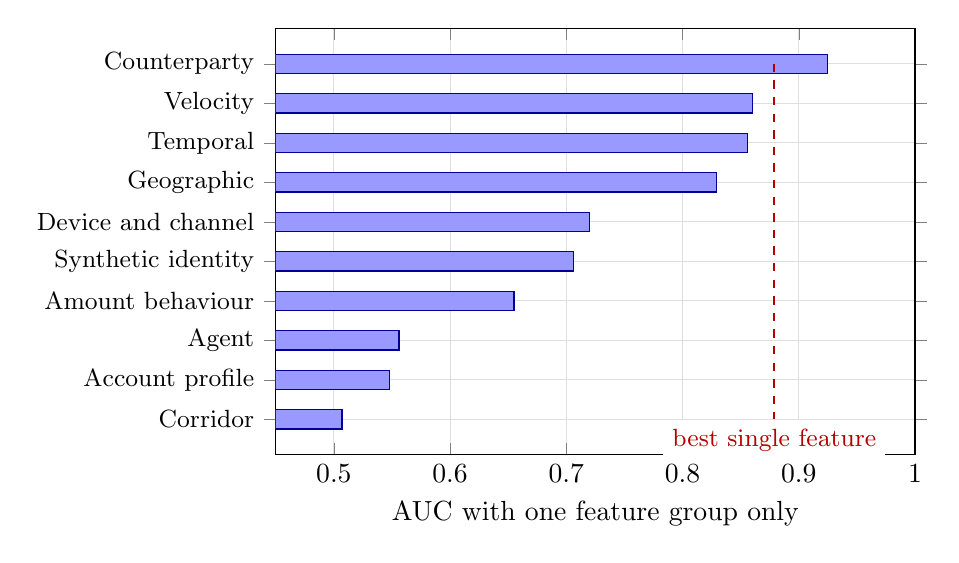
\begin{tikzpicture}
  \begin{axis}[
      width=0.8\linewidth, height=7cm,
      xbar, bar width=7pt, xmin=0.45, xmax=1.0,
      xlabel={AUC with one feature group only},
      symbolic y coords={{Counterparty},{Velocity},{Temporal},{Geographic},{Device and channel},{Synthetic identity},{Amount behaviour},{Agent},{Account profile},{Corridor}},
      ytick=data, y dir=reverse, yticklabel style={font=\small},
      grid=major, grid style={gray!25},
    ]
    \addplot[fill=blue!40, draw=blue!60!black] coordinates {(0.925,{Counterparty}) (0.86,{Velocity}) (0.856,{Temporal}) (0.829,{Geographic}) (0.72,{Device and channel}) (0.706,{Synthetic identity}) (0.655,{Amount behaviour}) (0.556,{Agent}) (0.548,{Account profile}) (0.507,{Corridor})};
    \draw[red!70!black, thick, dashed] (axis cs:0.879,{Counterparty}) -- (axis cs:0.879,{Corridor})
      node[pos=1, anchor=north, font=\small, fill=white] {best single feature};
  \end{axis}
\end{tikzpicture}

\caption{AUC of the diagnostic model with one feature group only (Table~\ref{tab:groups}), against the
best single feature on the same test rows (\nGateFloor{}, dashed). Four groups reach at least
\nGroupGeographic{} alone. Generated by \texttt{figures/make\_figures.py} from \texttt{numbers.tex}.}
\label{fig:groups}
\end{figure}

The benchmark can be solved several different ways, so no single group is load-bearing and a
leave-one-group-out ablation reports each as nearly free. This is a result about how a
scenario-driven generator encodes signal: a generator that plants fraud as incidents writes the
same structure into the velocity, counterparty, temporal and geographic views at once. On the
earlier draw \texttt{6abde44e} the same four groups each reached at least \nEarlyGroupMin{}; the
threshold moved with the draw and the finding did not.

It also disposes of a planned experiment. The specification's claim that models built elsewhere
reach far lower AUC on East African mobile money data is unverified (claims register, C-4), and
the proposed replacement, a card-style feature set against the full set, cannot answer it here:
the production ensemble restricted to card-style features changes AUC by \nAblCardD{}, and on a
benchmark this redundant a subset comparison shows a small difference whatever is true of real
systems. The specification's other ablations of the production ensemble are equally small
(without agent features \nAblAgentD{}, without the corridor feature \nAblCorridorD{}, without
round-sum awareness \nAblRoundD{}, without month-end awareness \nAblMonthD{}, without USSD-aware
device handling \nAblUSSDD{}) and are reported for completeness, not as evidence of what matters
in production.

\subsection{Calibration and explanation}

The row-weighted calibration error is nearly meaningless at a base rate below one per cent: almost every
row sits in the lowest bin, where no decision is made. On the diagnostic model we therefore also
report it in the decision region (score at or above the flag threshold, \nBatDecisionRows{} rows):
\nBatECEDecision{}, against \nBatECEAll{} over all rows. The additivity error of the exact TreeSHAP
contributions, which must sum to the model's margin, is \nBatAdditivity{}.

\subsection{The latency--explainability frontier}
\label{sec:frontier}

Resolution D-16 makes tree complexity a constrained hyperparameter: a configuration whose
single-request 99th-percentile latency, model plus exact TreeSHAP, exceeds 40~ms is rejected.
Table~\ref{tab:frontier} is the trade-off, measured one request at a time (a batch would amortise
exactly the overhead a single request pays), \nFrRequests{} timed requests per configuration after
a warm-up, on the development laptop.

\begin{table}[htbp]
\centering
\caption{Accuracy and median single-request latency across tree complexity (one XGBoost booster,
draw \texttt{6abde44e}, \nFrHeldOutRows{} held-out rows holding \nFrHeldOutFraud{} fraud,
\nFrRequests{} timed requests per configuration, evidence commit \texttt{95b722c}, source
\texttt{docs/benchmarks/m4\_frontier\_6abde44e.txt}). Milliseconds
are from the development laptop and are not gate figures (ADR 0010).}
\label{tab:frontier}
\begin{tabular}{rrrrrr}
\toprule
Trees & Depth & AUC & Predict p50 (ms) & With SHAP p50 (ms) & SHAP cost (ms) \\
\midrule
50 & 3 & \nFrAucA & \nFrPredA & \nFrShapA & \nFrCostA \\
100 & 4 & \nFrAucB & \nFrPredB & \nFrShapB & \nFrCostB \\
200 & 5 & \nFrAucC & \nFrPredC & \nFrShapC & \nFrCostC \\
400 & 6 & \nFrAucD & \nFrPredD & \nFrShapD & \nFrCostD \\
800 & 8 & \nFrAucE & \nFrPredE & \nFrShapE & \nFrCostE \\
\bottomrule
\end{tabular}
\end{table}

\begin{figure}[htbp]
\centering
% Generated by figures/make_figures.py from numbers.tex; do not edit.
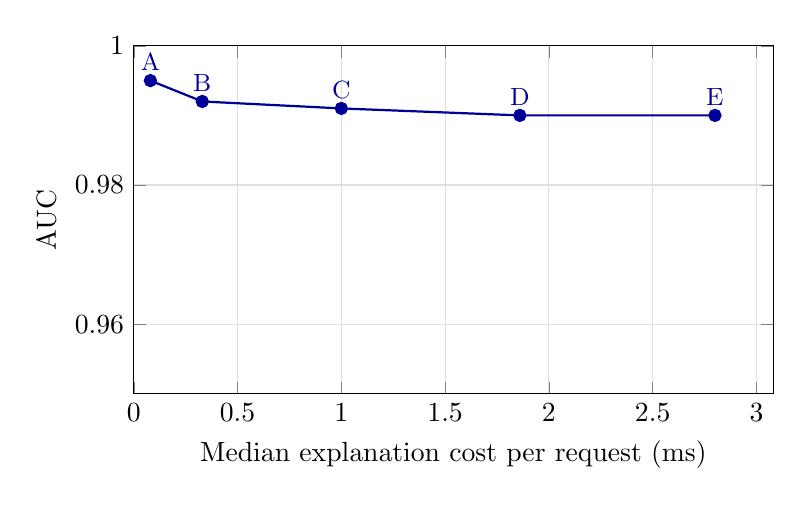
\begin{tikzpicture}
  \begin{axis}[
      width=0.8\linewidth, height=6cm,
      xlabel={Median explanation cost per request (ms)},
      ylabel={AUC}, ymin=0.95, ymax=1.0, xmin=0,
      grid=major, grid style={gray!25},
      nodes near coords, point meta=explicit symbolic,
      every node near coord/.append style={font=\small, anchor=south},
    ]
    \addplot[mark=*, thick, blue!60!black] coordinates {
      (0.08, 0.995) [A]
      (0.33, 0.992) [B]
      (1.0, 0.991) [C]
      (1.86, 0.99) [D]
      (2.8, 0.99) [E]
    };
  \end{axis}
\end{tikzpicture}

\caption{The frontier of Table~\ref{tab:frontier}: AUC against the median cost of an exact TreeSHAP
explanation, one point per configuration (A: the smallest, E: the largest). Accuracy stays within
its interval while the cost grows. Generated by \texttt{figures/make\_figures.py} from
\texttt{numbers.tex}.}
\label{fig:frontier}
\end{figure}

From the smallest configuration to the largest, AUC moves \nFrontAUCDelta{}, inside every
interval, while the median cost of explaining a decision grows about \nFrontRatio-fold, from
\nFrontShapSmall{} to \nFrontShapLarge{}~ms; prediction alone grows from \nFrontPredSmall{} to
\nFrontPredLarge{}~ms. The accuracy half is a property of this easy benchmark and should not be
generalised. The latency half is a property of the model and the explanation algorithm: exact
TreeSHAP costs $O(TLD^2)$ for $T$ trees with at most $L$ leaves and depth $D$
\cite{lundberg2020trees}, which is why an easy benchmark cannot weaken it.

Three cautions keep this result in proportion. First, every configuration explains a decision in a
few milliseconds at the median, far inside the specification's 40~ms per-request budget, so on this
evidence explanation cost binds at throughput (the work each core does per explained request)
rather than at the latency of a single request. Second, the \nFrontRatio-fold ratio depends on the
grid: it is measured from the cheapest configuration tried, and a different smallest configuration
would give a different ratio; the growth with trees and depth is the finding, not the number.
Third, it is one machine's median. On data like this, the explanation budget, not the accuracy
target, should choose the tree configuration.

\textbf{We report the median only.} In \nFrontNegative{} configurations the measured 99th
percentile shows a \emph{negative} explanation cost, which is impossible: explaining cannot be
faster than not explaining. The tail on this shared machine is scheduler jitter, not model
complexity. D-16's 40~ms constraint therefore cannot be applied from this run; the
99th-percentile frontier on a dedicated machine is \notyet{M10}. Three further limits: one model
family (not the ensemble), one process (not the specified multi-process service), and a SHAP cost
paid on every row, whereas in serving it is paid only on flagged transactions.

\subsection{What this evaluation does not yet report}

\begin{itemize}
  \item Precision at a fixed analyst alert budget, the operational number: \notyet{M4 follow-up}.
  \item Performance by month of the test period (claims register, C-5): \notyet{M4 follow-up}.
  \item The cost curve of fraud loss prevented against legitimate transactions blocked and
        reviews required: \notyet{M4 follow-up}.
  \item Leave-one-fraud-type-out and the value of Isolation Forest routing for novelty:
        \notyet{M4 follow-up}.
  \item Shadow-mode AUC delta and scoring latency of the serving path: \notyet{M5}.
  \item End-to-end decision latency and throughput at the specified load: \notyet{M6 and M10}.
\end{itemize}

\section{Generalisation: two nulls and one failure}
\label{sec:generalisation}

Once a single feature reached \nFloorM{}, the headline AUC could no longer show that a model had
learned anything a one-line rule could not. Two experiments were meant to carry that weight
instead: leave-one-country-out, and a fraud sub-variant that appears only in the test period.
Both are null. This section reports them as null results rather than dropping them, explains why
this benchmark could not make them informative, and reports the one experiment that did find a
failure.

\subsection{Leave-one-country-out}

Each country is removed from training entirely and then scored, and each result is compared with
the same country scored by the model that saw it (Table~\ref{tab:loco}). Removing a country costs
at most \nLocoMaxLoss{} AUC; on the earlier draw \texttt{6abde44e} it cost at most
\nEarlyLocoMaxLoss{}.

\begin{table}[htbp]
\centering
\caption{AUC per country, in-sample and with the country unseen in training (diagnostic model,
draw \texttt{d8083dbc}, \nBatTestRows{} test rows, evidence commit \texttt{d40fca2}, source
\texttt{docs/benchmarks/m4\_battery\_d8083dbc\_e1.txt}). CD rests
on fewer than 30 fraud rows and gives direction only.}
\label{tab:loco}
\begin{tabular}{lrrr}
\toprule
Country & In-sample & Unseen in training & Fraud rows \\
\midrule
KE & \nLocoKEin & \nLocoKEout & \nLocoKEf \\
RW & \nLocoRWin & \nLocoRWout & \nLocoRWf \\
TZ & \nLocoTZin & \nLocoTZout & \nLocoTZf \\
UG & \nLocoUGin & \nLocoUGout & \nLocoUGf \\
CD & \nLocoCDin & \nLocoCDout & \nLocoCDf \\
\bottomrule
\end{tabular}
\end{table}

The null has a mechanism, and it is tested rather than argued: \textbf{no fraud parameter is keyed
by country} (a test fails if one is). Country enters only as a lookup for which mule, merchant,
agent, currency or time zone an incident uses, so withholding a country withholds no fraud
mechanism. Country-level generalisation cannot be evaluated on this benchmark and belongs to a
real-data validation plan. We did not change the generator to make countries differ: no source
read gives fraud prevalence by type and country for these markets, so the only way to choose such
a parameter would be to pick whatever makes the experiment show a gap, which defines the ground
truth from the test's desired answer (ADR 0028).

\subsection{A novel variant held out in time}

\texttt{novel\_esim\_delayed\_drain} occurs only in the test period. All variants are scored
against the same legitimate rows at one threshold, the \nFPRBudget{} false-positive budget over all
legitimate rows. The unseen variant is caught at \nNovelRecall{} \nNovelCI{} (\nNovelCaught{} of
\nNovelRows{}), against \nBaseVarRecall{} \nBaseVarCI{} for the base scenarios the model trained
on: at least as often as the familiar shape. On the earlier draw the figures were
\nEarlyNovelRecall{} against \nEarlyBaseRecall{}. The variant's novelty is in its lead time (a
drain delayed by days rather than minutes after the enabling SIM event), not in its transaction
pattern, which is still a burst, so a model that detects bursts catches it without having seen it.
This is not an out-of-distribution test.

\subsection{One cause}

Both nulls, and the redundancy of Section~\ref{sec:redundancy}, have one explanation: \textbf{the
benchmark encodes fraud as bursts}, and every country, every variant and every feature group is a
view of that single structure. What the benchmark supports is detection \emph{given}
burst-structured fraud, and the cost of computing and explaining that detection. It supports no
claim about generalisation, geographic or temporal.

\subsection{A pre-registered non-burst variant: the one failure found}

A generalisation test needs a mechanism that actually differs, and the ``sent by mistake'' reversal
scam is one. Its ingredients are documented among Kenyan M-PESA users. In a survey of them,
forged M-PESA confirmation messages were the most common scam reported \cite[Section~5.1.1]{dogan2025grift};
the same study notes that M-PESA's business services block reversals to foil opportunistic and
malicious reversal requests \cite[Section~2]{dogan2025grift}, and one respondent reported asking
the sender to reverse an apparently mistaken transfer \cite[Section~5.3.3]{dogan2025grift}. The scam itself
is described in the Kenyan press: the victim receives a fake M-PESA message that shows ``LOCKED''
where the balance should be, the scammer claims to have sent the money by mistake, often with an
emotional story, and the victim sends it back, only to find that no money was ever deposited;
Safaricom's advice, quoted there, is not to refund the money \cite{star2025mpesa}. The victim's
loss is therefore a single transfer that the victim initiates, to the number of the claimed sender.
Neither source says whether the victim has paid that number before; since it is the scammer's own
number, we read the documented form as a transfer to a new counterparty.

The benchmark's variant keeps the single, victim-initiated transfer and departs from that form in
one deliberate respect: its recipient is a counterparty the victim already knows. That is a
modelling choice, not a property the sources describe (ADR 0028). It removes both axes this
benchmark's detection relies on at once, burst structure and counterparty novelty, which makes the
variant the harder case of the two: the documented form, with its new recipient, keeps counterparty
novelty. The generator stages each such row as a \texttt{mule\_account} row with its own sub-variant
label (Table~\ref{tab:scenarios}).

The variant's definition, its justification and the predicted result were committed before the
dataset was regenerated and before any measurement existed (ADR 0028). The prediction: recall at
the same threshold \textbf{between \nRevPredLow{} and \nRevPredHigh{}}, lower than the base
scenarios but not zero, with recall below about \nRevPredFloor{} stated as the outcome that would
say burst structure and counterparty novelty carry nearly all of the benchmark's detection power.

\textbf{Result.} \texttt{reversal\_scam\_social\_engineering} is caught at \nRevRecall{}
(\nRevCaught{} of \nRevFraud{}, Wilson \nRevCI{}), against \nBaseVarRecall{} \nBaseVarCI{} for the
base scenarios on \nBaseVarFraud{} rows; its AUC is \nRevAUC{}. The intervals do not overlap.
The denominator is \nRevFraud{} rather than the \nRevRows{} rows the generator wrote because the
evaluation reads the observed label, as a deployed model would: all \nRevTrueFraud{} rows are in
the test period and are fraud by their true label, and \nRevScoredUnlabelled{} of them carry the
benchmark's missed-fraud label noise (Section~\ref{sec:dataset}), so they are scored as legitimate
rows (\texttt{evidence/\allowbreak reversal\_\allowbreak labels\_\allowbreak d8083dbc.txt},
Appendix~\ref{app:evidence}). The
point estimate is below the pre-registered range; the interval now reaches past the range's lower
edge, so ``below the predicted range'' holds for the point estimate and not for the whole interval.

\begin{figure}[htbp]
\centering
% Generated by figures/make_figures.py from numbers.tex; do not edit.
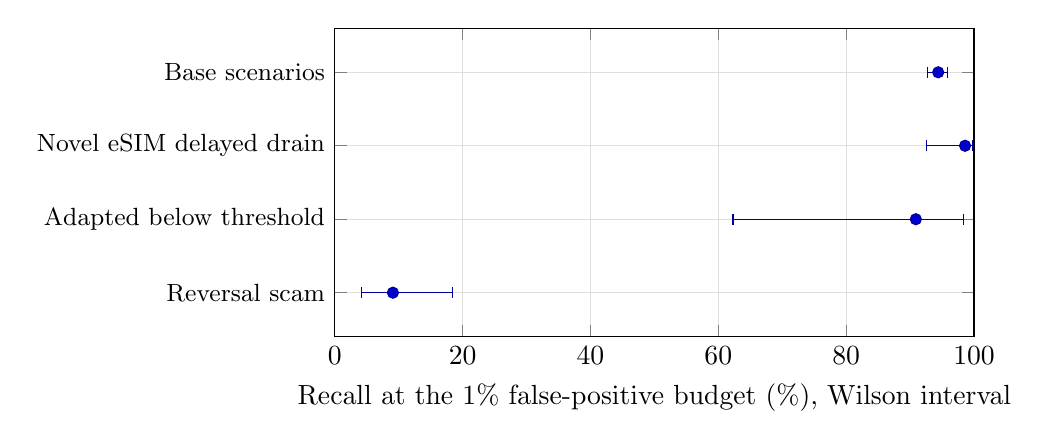
\begin{tikzpicture}
  \begin{axis}[
      width=0.8\linewidth, height=5.5cm,
      xmin=0, xmax=100, xlabel={Recall at the 1\% false-positive budget (\%), Wilson interval},
      symbolic y coords={{Base scenarios},{Novel eSIM delayed drain},{Adapted below threshold},{Reversal scam}},
      ytick=data, y dir=reverse, yticklabel style={font=\small}, enlarge y limits=0.2,
      grid=major, grid style={gray!25},
    ]
    \addplot+[only marks, mark=*, blue!60!black,
      error bars/.cd, x dir=both, x explicit] coordinates {
      (94.4,{Base scenarios}) -= (1.7,0) += (1.4,0)
      (98.6,{Novel eSIM delayed drain}) -= (6.0,0) += (1.2,0)
      (90.9,{Adapted below threshold}) -= (28.6,0) += (7.5,0)
      (9.1,{Reversal scam}) -= (4.9,0) += (9.3,0)
    };
  \end{axis}
\end{tikzpicture}

\caption{Recall of each fraud variant at the same threshold, with Wilson intervals (diagnostic
model, draw \texttt{d8083dbc}, \texttt{docs/benchmarks/m4\_battery\_d8083dbc\_e1.txt}). Generated by
\texttt{figures/make\_figures.py} from \texttt{numbers.tex}.}
\label{fig:variants}
\end{figure}

\textbf{A correction, reported rather than hidden.} The first measurement gave \nRevRecallFirst{}
\nRevCIFirst{} (\nRevCaughtFirst{} of \nRevFraud{}; AUC \nRevAUCFirst{}) against
\nBaseVarRecallFirst{} \nBaseVarCIFirst{}. It used a random-fold target encoding, which the project's rule that
every fold, split, sample and encoding groups by account (E1) forbids; re-running on the same data with the permitted encoding produced the
figures above. The conclusion did not change; the interval did.

\textbf{What this does and does not show.} It confirms, on a held-out shape rather than by inference
from ablation margins, that when burst structure and counterparty novelty are both absent the
remaining signals (amount, channel, time) do not recover this benchmark's detection power. Because
the variant removes the two axes together, the result cannot say how much each contributes on its
own; a variant with a new recipient, as in the documented form, would separate them and has not
been measured. It does not show that non-burst fraud is undetectable: other typologies are
untested, and a real system has signals this benchmark does not simulate. A second
held-out variant, \texttt{adapted\_below\_threshold}, rests on \nAdaptFraud{} fraud rows (recall
\nAdaptRecall{} \nAdaptCI{}); its interval overlaps the base scenarios' and establishes nothing on
its own.

\section{Discussion}
\label{sec:discussion}

The project kept a lab notebook (\texttt{docs/research/lab\_notebook.md}) in which every defect,
correction and prediction was written down when it happened and never edited afterwards; later
corrections are new entries. This section is built from it. Its value is not that the benchmark
is good, but that the ways a careful process still went wrong are recorded, and several recur.

\subsection{Recurring failure patterns}

\paragraph{A control measured on the inputs is not a control on the system.} The most frequent
pattern, recorded under several names (``a guard with two doors'', ``a fix that keeps the old
behaviour as a floor''). A parameter digest guarded the generator's inputs while the claim lived
in its output: the draw could change with every parameter identical, which is why datasets are now
identified by a fingerprint over their rows. A statistical band kept a fixed floor that, at release
scale, was several times wider than the band it was meant to bound, so the check could not fail.
Out-of-fold encoding removed each row's own label but left the other rows of the same fraud
incident in the estimate, inflating every single-feature AUC by about \nSiblingLeak{} until folds
were grouped by account; later, account grouping turned out not to protect features whose unit of
history is a counterparty or a map cell. The single-column separation ceiling was true of the columns it
measured and false of the engineered features it was quoted about. The fingerprint fix itself first hashed only some of
the columns. In each case the obvious form of the defect (the individual value, the row) was
fixed and the aggregate form (the set, the group, the regime) was not. The habit that follows,
now an exit criterion: for every guard, name the object it ranges over and read the sentence it
is supposed to justify; if the nouns differ, it does not justify the sentence. And prefer a guard
with no scope parameter to one with a well-chosen scope.

\paragraph{An asserted protection is worse than a missing one.} A documented cross-account control
that did not in fact control anything, and a code comment explaining why a truncated corpus could
not bias a feature, both survived review by being reassuring rather than invisible. The comment's
argument turned out to be right for the feature it named, and was only established once it was
measured (Section~\ref{sec:floor}); the search it prompted found three further features with the
flaw the comment had ruled out for its own. Controls must now name the mutation that would detect their failure, and the
rule recorded is that an aggregate over a window can be derived from a corpus, while a statement
about all of history cannot.

\paragraph{A test that cannot fail proves nothing.} Fixtures built to be small rather than to
contain the condition under test passed vacuously: a fold test whose categories were pure, a drift
test whose fixture had no drifting rows. Tests now assert their precondition before their
conclusion, and fixtures are specified by the property they must have before their size.

\paragraph{The wrong denominator.} The central methodological error of the dataset milestone was
standardising a detector's offset against a theoretical null rather than the observed seed-to-seed
spread; a
single three-sigma reading turned out to be noise once repeated seeds were run. The first model margin
reported subtracted a feature measured on a few hundred rows holding two frauds from a model
measured on the full test set. Every baseline now prints the rows and fraud it rests on, and a
partial-coverage feature is never subtracted from a model.

\paragraph{Records that run ahead of the facts.} A status table marked a gate as met by citing a
run that did not exist; an evidence file attributed to a commit had been produced from a dirty
working tree; a milestone tag was placed on a commit whose continuous integration had not passed.
Each is a hand-written summary of a machine-checkable fact, drifting in the flattering direction.
Status is now derived from the existence of evidence artefacts, evidence files carry the tree
state they were produced from, and a tag requires a green run on the exact commit.

\paragraph{Knowing a failure mode does not immunise against it.} Several of these patterns recurred
after they had been analysed and recorded. The lesson
the notebook draws is that a defence that depends on remembering a rule at the moment of temptation
is not a defence; each lesson is useful only with the question ``what would enforce this?''
attached, and most of the rules above are now tests.

\paragraph{A hedge is often an unmeasured claim.} Several caveats (``the delay channel might be
mostly an artefact'', ``burstiness is not country-specific'') turned out to be measurable, and
measuring them replaced a hedge with a result: about \nEventDelayShare{} of the delay channel was
artefact, and leave-one-country-out is null. The test for keeping a caveat is to ask what
measurement would remove it.

\subsection{Pre-registered predictions}

The notebook recorded \nPredTotal{} falsifiable predictions before the evidence existed, and
reports each outcome where the prediction was made, whether confirmed or refuted
(Table~\ref{tab:predictions}).

\begin{table}[htbp]
\centering
\small
\caption{Pre-registered predictions and outcomes, from the lab notebook.}
\label{tab:predictions}
\begin{tabular}{p{0.52\linewidth}p{0.38\linewidth}}
\toprule
Prediction & Outcome \\
\midrule
Shortcut-detector power dips when the eighth scenario appears above the minimum scale &
Refuted: power rose monotonically, no dip \\
The detector's small positive offset is real and constant with scale &
Refuted: pooled over seeds, the interval straddles chance \\
A counterparty-keyed feature will force an eighth field into the feature contract &
Confirmed on mechanism, wrong on sequence \\
\texttt{accounts\_per\_device\_7d} cannot be made fold-safe without an owner decision &
Refuted: grouping accounts that share a device resolves it \\
A long-tailed takeover lead lowers the event-delay channel to
\nEventDelayBandLow{}--\nEventDelayBandHigh{} &
Confirmed: \nEventDelayAfter{}, at the top of the band \\
The reversal scam is caught at \nRevPredLow{}--\nRevPredHigh{} recall &
Refuted: \nRevRecall{} \nRevCI{}; below the range for the point estimate, not for the whole
interval \\
\bottomrule
\end{tabular}
\end{table}

Of the first \nPredEarly{}, \nPredEarlyRight{} was partly right. The claim this supports is not that
the author predicted well. It is that falsifiable predictions were recorded before the evidence,
that most were wrong, that each refutation cost a paragraph rather than a shipped result, and that
several of the guards now in the system exist because of what the refutations found.

\subsection{A benchmark audit protocol}

The checks below are what we would run before trusting any synthetic benchmark, whoever built it.
Each one exists because its absence hid something here: Table~\ref{tab:protocol} states what each
check detects and what it found on FraudShield-EAC. They are cheap: every one is a measurement on
data that already exists, and together they decide which claims the benchmark can carry.

\begin{table}[htbp]
\centering
\small
\caption{A benchmark audit protocol: the checks, what each detects, and what each found on
FraudShield-EAC. Every finding is reported in the section named.}
\label{tab:protocol}
\begin{tabular}{p{0.26\linewidth}p{0.3\linewidth}p{0.36\linewidth}}
\toprule
Check & What it detects & What it found here \\
\midrule
The best single \emph{engineered} feature, not only the best raw column &
A benchmark one rule can solve, and model metrics quoted against chance &
The velocity ratio alone reaches \nFloorM{}, while the strongest raw column reaches
\nColumnMaxAUCB{}; every metric is now a margin over the floor (Section~\ref{sec:floor}) \\
\addlinespace
Leave-one-group-out \emph{and} one-group-only &
Redundancy read as irrelevance: the first check alone cannot tell them apart &
Removing any group costs at most \nGroupMaxDrop{}, yet four groups each reach at least
\nGroupGeographic{} alone (Section~\ref{sec:redundancy}) \\
\addlinespace
Does each generalisation experiment withhold a \emph{mechanism}, or only a label? &
Experiments that cannot fail, reported as evidence of generalisation &
No fraud parameter is keyed by country, so leave-one-country-out costs at most \nLocoMaxLoss{};
the variant held out in time is still a burst and is caught at \nNovelRecall{}
(Section~\ref{sec:generalisation}) \\
\addlinespace
A pre-registered variant from an independently documented typology &
Whether detection survives without the benchmark's dominant structure &
Recall \nRevRecall{} \nRevCI{} against \nBaseVarRecall{} \nBaseVarCI{}, below the registered
prediction (Section~\ref{sec:generalisation}) \\
\addlinespace
A fingerprint over the output rows, beside any digest of the parameters &
Reports that silently describe a different draw &
A refactor that changed no parameter value re-drew the whole benchmark; datasets are now
identified by their rows (Section~\ref{sec:repro}) \\
\addlinespace
Encodings and folds grouped by each feature's unit of history &
Leakage between rows of one incident, which inflates every feature's score &
Out-of-fold encoding grouped by row inflated single-feature AUC by \nSiblingLeak{}; grouping by
account fixed it, and features keyed by counterparty or map cell needed their own grouping \\
\addlinespace
For every control, a named mutation that would kill it &
Controls and tests that cannot fail &
Vacuous fixtures (a fold test with pure categories, a drift test with no drift) and a documented
cross-account control that controlled nothing \\
\bottomrule
\end{tabular}
\end{table}

On FraudShield-EAC each of these changed what could be claimed.

\section{Ethics, fairness and privacy}
\label{sec:ethics}

\paragraph{Who bears the errors.} A false positive in this system declines or holds a legitimate
payment. For a customer who depends on a mobile money transfer for wages, school fees or a family
remittance, a blocked payment is a real harm, and it falls hardest on customers with the least
slack: low balances, basic handsets, and (because USSD carries no device signals) the channel
where the model has least to go on. The specification therefore requires a fairness report
(build prompt E.5 item 7): false-positive rate and blocked legitimate amount by country, channel,
KYC tier and urban or rural location. That report is \notyet{M4 follow-up}. The per-country and
per-channel AUCs in Sections~\ref{sec:evaluation} and~\ref{sec:generalisation} are not a fairness
analysis: they measure ranking, not who is wrongly blocked. On a synthetic benchmark whose
population structure is partly sourced and whose fraud is assumed, even the fairness report will
describe the generator's disparities, not a real population's.

\paragraph{Customer verification.} The specification's self-service unblocking by SMS link would
be defeated by the fraud it targets: in a SIM-swap takeover the attacker holds the victim's SIM and
receives the link. Self-service is therefore disabled when a SIM swap is recent or its recency is
unknown, when the device changed in the last day, or when the score is very high, and the customer
is directed to the institution's official number (resolution D-25). This is specified behaviour of
a later milestone, not an evaluated result.

\paragraph{Privacy.} The benchmark contains no real personal data. The system is specified to keep
personal data out of every analytic path: account, device and counterparty identifiers are opaque
tokens, raw phone and account numbers are rejected at ingestion, and personal data lives only in a
separate encrypted vault (resolution D-20). Logs are required to pass through redacting processors.
Explanations shown to analysts and customers are specified to come from deterministic
templates, never from a language model.

\paragraph{Regulation and residency.} Statements about reporting obligations and data protection
in Rwanda (for example the data protection law and the financial intelligence reporting framework)
are unverified and must be confirmed by a compliance professional (resolution D-22); report
templates carry fields marked as unconfirmed. Production data must reside in a facility that is
legally permitted for it; the infrastructure code cannot satisfy that requirement, and
demonstration environments run on synthetic data only, labelled as such (resolution D-21).

\paragraph{What this paper does not claim.} That FraudShield is deployed at, endorsed by, or
validated with any real institution or regulator, or that any figure here predicts performance on
real transactions.

\section{Limitations}
\label{sec:limitations}

We state these as findings about what the evidence supports, not as disclaimers.

\paragraph{The benchmark is synthetic, and the fraud in it is invented.} It supports comparisons
between methods under identical conditions. It does not support statements about real fraud rates,
real detection performance or any institution's customers. Every figure here is a property of this
generator.

\paragraph{No fraud parameter is sourced.} Of \nFraudParams{} fraud parameters,
\nFraudParamsChoice{} are modelling choices and \nFraudParamsCalibrated{} are calibrated to
specification targets. No publication read gives fraud incidence by type for these markets. Any
result that depends on the level or mix of fraud, rather than on the relative ordering of methods,
inherits this assumption. The sourced parameters (\nParamsSourced{} of \nParamsTotal{}) fix
population and volume structure, partly from a neighbouring market's statistics.

\paragraph{The benchmark is burst-separable.} Its fraud is injected as bursts, so a single velocity
feature reaches \nFloorM{}, four feature groups each nearly solve it alone, leave-one-country-out
and the novel variant are both null, and the one pre-registered non-burst variant is almost
invisible to the model. Detection of burst-structured fraud is what the benchmark measures; nothing
here speaks to fraud with other structure, except as the failure in
Section~\ref{sec:generalisation}. The specification's distribution targets (overall and test-period
fraud rate, channel and country mix) are requirements met by construction, not observations.

\paragraph{No real-data validation.} None has been done. A validation on real data would need to
show, at minimum: the single-feature floor on real engineered features (whether real fraud is as
burst-separable as this benchmark's); the ensemble's margin over that floor; calibration in the
decision region; leave-one-country-out on real, country-labelled fraud; and detection of
documented non-burst typologies such as the reversal scam. It would require data access agreements,
a data protection impact assessment, and hosting in a permitted location (Section~\ref{sec:ethics}).

\paragraph{Scale and volume.} Results are at about one million rows, not the five million the
specification requires (\notyet{M10}), and the models were trained on \nTrainUsed{} rows rather than
the full training period. Single-feature AUC moves with dataset size by more than seed noise, and the
cause is unexplained; every figure is therefore stated at its scale. The two failing gate metrics
(recall and false-negative rate at the flag threshold) may depend on training volume; that is a
candidate cause, not a finding.

\paragraph{Latency.} No latency figure here is a gate figure. The frontier is a median on a shared
development laptop, where the 99th percentile is not measurable; serving, end-to-end and load
latencies belong to later milestones.

\paragraph{Small counts.} Variant, country and channel results rest on tens to hundreds of fraud
rows; intervals are reported for each, and the Democratic Republic of the Congo's rest on fewer than
30 and give direction only.

\paragraph{Provisional results.} Every figure marked \textsuperscript{\dag} comes from a milestone not
yet tagged complete and is re-verified before publication. Two of the contribution figures already
moved between data draws (the redundancy threshold and the leave-one-country-out loss); the findings
did not.

\paragraph{Claims not made.} The specification's figures on regional fraud growth, payment volume,
analyst dismissal rates, the accuracy of models built elsewhere on East African data, annual model
degradation and ensemble variance reduction are unverified, replaced or refuted in the project's
claims register, and none is stated here as fact.

\section{Reproducibility statement}
\label{sec:repro}

\paragraph{Data.} The benchmark is generated, not distributed as a fixed file: seed \nSeed{} and
the generator code at a stated commit reproduce a draw byte for byte, independently of how the work
is batched. Each draw is identified by a SHA-256 fingerprint over its output rows (\texttt{6abde44e}
and \texttt{d8083dbc} in this paper), and its realism report records the parameter hash, the check
set hash and the fingerprint. The dataset release is licensed CC BY 4.0
(\texttt{dataset/release/}); the code is Apache-2.0.

\paragraph{Evidence.} Every figure in this paper comes from a raw output file (Appendix~\ref{app:evidence}) under
\texttt{docs/benchmarks/} whose header records the command, its exit status, the commit and whether
the working tree was clean; \texttt{numbers.tex} maps each figure in the text to its file. Every
read of the test period is logged in \texttt{docs/benchmarks/test\_set\_access.jsonl}. Experiment
tracking in MLflow was not used for the evidence in this paper (ADR 0030); the evidence files carry the
provenance instead.

\paragraph{Hardware.} All measurements were made on one development laptop (\nHwCPU{},
\nHwMem{}), recorded in \texttt{docs/benchmarks/hardware.md}. Latency figures from it are reported
as shapes, not as gate numbers (ADR 0010).

\paragraph{One command.} A single target that regenerates the dataset, trains, evaluates and
produces the paper's tables and figures from a clean machine, with compute time and hardware
recorded, is \notyet{M11}. Until it exists, each figure is reproduced by the command recorded in its
evidence file.

\paragraph{Publication.} Scripts and checklists for publishing the dataset and model, for the author
to run, are part of this milestone and do not exist yet. No DOI exists, and none is cited.


\bibliographystyle{plain}
\bibliography{references}

\end{document}
